\PassOptionsToPackage{unicode}{hyperref}
\PassOptionsToPackage{naturalnames}{hyperref}
\PassOptionsToPackage{table}{xcolor}

\documentclass[14pt]{beamer}

\mode<presentation> {

% The Beamer class comes with a number of default slide themes
% which change the colors and layouts of slides. Below this is a list
% of all the themes, uncomment each in turn to see what they look like.

%\usetheme{default}
%\usetheme{AnnArbor}
%\usetheme{Antibes}
%\usetheme{Bergen}
%\usetheme{Berkeley}
%\usetheme{Berlin}
%\usetheme{Boadilla}
%\usetheme{CambridgeUS}
%\usetheme{Copenhagen}
%\usetheme{Darmstadt}
%\usetheme{Dresden}
%\usetheme{Frankfurt}
%\usetheme{Goettingen}
%\usetheme{Hannover}
%\usetheme{Ilmenau}
%\usetheme{JuanLesPins}
%\usetheme{Luebeck}
%\usetheme{Madrid}
%\usetheme{Malmoe}
%\usetheme{Marburg}
%\usetheme{Montpellier}
%\usetheme{PaloAlto}
%\usetheme{Pittsburgh}
%\usetheme{Rochester}
%\usetheme{Singapore}
%\usetheme{Szeged}
%\usetheme{Warsaw}

% As well as themes, the Beamer class has a number of color themes
% for any slide theme. Uncomment each of these in turn to see how it
% changes the colors of your current slide theme.

%\usecolortheme{albatross}
%\usecolortheme{beaver}
%\usecolortheme{beetle}
%\usecolortheme{crane}
%\usecolortheme{dolphin}
%\usecolortheme{dove}
%\usecolortheme{fly}
%\usecolortheme{lily}
%\usecolortheme{orchid}
%\usecolortheme{rose}
%\usecolortheme{seagull}
%\usecolortheme{seahorse}
%\usecolortheme{whale}
%\usecolortheme{wolverine}

%\setbeamertemplate{footline} % To remove the footer line in all slides uncomment this line
%\setbeamertemplate{footline}[page number] % To replace the footer line in all slides with a simple slide count uncomment this line

\setbeamertemplate{navigation symbols}{} % To remove the navigation symbols from the bottom of all slides uncomment this line
\setbeamertemplate{frametitle continuation}[from second][(\insertcontinuationcountroman)]
}

\usepackage{graphicx} % Allows including images
\usepackage{booktabs} % Allows the use of \toprule, \midrule and \bottomrule in tables
%\usepackage[T1]{fontenc}
\usepackage[spanish]{babel}
\usepackage[utf8]{inputenc}
\usepackage{listings}
\usepackage{tikz}
\usetikzlibrary{positioning,backgrounds}
\usetikzlibrary{decorations.pathmorphing,math}
%\usepackage{iwona}
%\usepackage{marvosym}
%\usepackage{cfr-lm}
%\usepackage{pifont}
%\usepackage{keystroke}
%\usepackage{etoolbox}

% Language Definitions for CYPHER
\lstdefinelanguage{cypher}{
morecomment=[l][\color{gray}]{//},
morestring=[b][\color{olive}]\",
morestring=[b][\color{olive}]\',
morekeywords={MATCH,WHERE,LIMIT,CREATE,RETURN,DISTINCT,DELETE,DETACH,UNIQUE,MERGE,INDEX,ON,SET,LOAD,CSV,FOREACH,IN},
sensitive=true
}

%
% Listados de código
%
\lstset{%
basicstyle=\ttfamily\footnotesize,
commentstyle=\color{gray}\itshape\ttfamily,
keywordstyle=\color{blue!80}\bfseries\ttfamily,
stringstyle = \color{gray},
showstringspaces=false,
frame=tblr, % single, tb, ltrb % boxed listings, en mayusculas = doble linea
framerule=0pt,
tabsize=4, % tabulador = 2 espacios
captionpos=b,
backgroundcolor=\color{yellow!20},
breaklines=true,
%backgroundcolor=\color{white},
%numbers=left, numberstyle=\tiny, stepnumber=2, numbersep=10pt,
xleftmargin=0.02\textwidth,
xrightmargin=0.02\textwidth,
language=java, % Por defecto
literate={«}{{\guillemotleft}}1
           {»}{{\guillemotright}}1
{á}{{\'a}}1 {é}{{\'e}}1 {í}{{\'i}}1 {ó}{{\'o}}1 {ú}{{\'u}}1
  {Á}{{\'A}}1 {É}{{\'E}}1 {Í}{{\'I}}1 {Ó}{{\'O}}1 {Ú}{{\'U}}1
  {à}{{\`a}}1 {è}{{\`e}}1 {ì}{{\`i}}1 {ò}{{\`o}}1 {ù}{{\`u}}1
  {À}{{\`A}}1 {È}{{\'E}}1 {Ì}{{\`I}}1 {Ò}{{\`O}}1 {Ù}{{\`U}}1
  {ä}{{\"a}}1 {ë}{{\"e}}1 {ï}{{\"i}}1 {ö}{{\"o}}1 {ü}{{\"u}}1
  {Ä}{{\"A}}1 {Ë}{{\"E}}1 {Ï}{{\"I}}1 {Ö}{{\"O}}1 {Ü}{{\"U}}1
  {â}{{\^a}}1 {ê}{{\^e}}1 {î}{{\^i}}1 {ô}{{\^o}}1 {û}{{\^u}}1
  {Â}{{\^A}}1 {Ê}{{\^E}}1 {Î}{{\^I}}1 {Ô}{{\^O}}1 {Û}{{\^U}}1
  {œ}{{\oe}}1 {Œ}{{\OE}}1 {æ}{{\ae}}1 {Æ}{{\AE}}1 {ß}{{\ss}}1
  {ű}{{\H{u}}}1 {Ű}{{\H{U}}}1 {ő}{{\H{o}}}1 {Ő}{{\H{O}}}1
  {ç}{{\c c}}1 {Ç}{{\c C}}1 {ø}{{\o}}1 {å}{{\r a}}1 {Å}{{\r A}}1
  {€}{{\euro}}1 {£}{{\pounds}}1
           {ñ}{{\~n}}1
           {Ñ}{{\~N}}1
           {¿}{{?`}}1
}

\colorlet{punct}{red!60!black}
\definecolor{background}{HTML}{EEEEEE}
\definecolor{delim}{RGB}{20,105,176}
\colorlet{numb}{magenta!60!black}

\lstdefinelanguage{json}{
    basicstyle=\ttfamily,
    stepnumber=1,
    numbersep=8pt,
    showstringspaces=false,
    breaklines=true,
%    frame=lines,
    moredelim=**[is][\color{red}]{@}{@},
    moredelim=**[is][\color{blue}]{º}{º},
%    backgroundcolor=\color{background},
    literate=
      {:}{{{\color{punct}{:}}}}{1}
      {,}{{{\color{punct}{,}}}}{1}
      {\{}{{{\color{delim}{\{}}}}{1}
      {\}}{{{\color{delim}{\}}}}}{1}
      {[}{{{\color{delim}{[}}}}{1}
      {]}{{{\color{delim}{]}}}}{1}
}

\definecolor{darkgray}{rgb}{.4,.4,.4}
\definecolor{purple}{rgb}{0.65, 0.12, 0.82}

\lstdefinelanguage{JavaScript}
{
  basicstyle=\ttfamily,
  keywords={typeof,new,true,false,catch,function,return,null,catch,switch,var,if,in,while,do,else,case
,break},
ndkeywords={class, export, boolean, throw, implements, import, this},
ndkeywordstyle=\color{darkgray}\bfseries,
sensitive=false,
comment=[l]{//},
morecomment=[s]{/*}{*/},
morestring=[b]',
morestring=[b]"
}

%% Macros comunes
\newcommand{\hide}[1]{}
\newcommand{\ra}{{\color{blue} $\Rightarrow${}~{}}}

\usepackage{fontspec}
\defaultfontfeatures{Ligatures=TeX,Numbers=OldStyle}
% \setmainfont{Aller_Lt.ttf}[
% BoldFont = Aller_Rg.ttf,
% ItalicFont = Aller_LtIt.ttf,
% BoldItalicFont = Aller_It.ttf]
\setsansfont
  [Ligatures=TeX, % recommended
   UprightFont={* Light},
   ItalicFont={* Light Italic},
   BoldFont={*},
   BoldItalicFont={* Italic}]
  {Open Sans}
% \setsansfont
%   [Ligatures=TeX, % recommended
%    UprightFont={* Regular},
%    ItalicFont={* Italic}]
%   {Fira Sans}
%\setmainfont{Open Sans}[BoldFont={* Bold}]
% \setmonofont[Ligatures = TeX,
% UprightFont={* Light},
%    ItalicFont={* Light Italic},
%    BoldFont={* Medium},
%    BoldItalicFont={* Medium Italic}]{Input Mono}

%\setmonofont{Input Mono}
\setmonofont%[Scale=1.1]
 % [Ligatures=TeX, % recommended
 %  UprightFont={* Regular},
 %  ItalicFont={* Italic},
 %  BoldFont={* Bold},
 %  BoldItalicFont={* Bold Italic}]
{Fira Mono}

\setbeamercolor{block title}{bg=blue!30,fg=black}
\setbeamercolor{block body}{bg=blue!20,fg=black}
\setbeamercolor{block title alerted}{bg=red!30,fg=black}
\setbeamercolor{block body alerted}{bg=red!20,fg=black}

\newsavebox{\mysubpic}

\usebackgroundtemplate{
%\setbox{\mysubpic}{
  \sbox{\mysubpic}{%
    \begin{tikzpicture}[remember picture,line width=1em,blue!30] %sub-picture
      \foreach \s in {1,...,\value{framenumber}}{
        \tikzmath{
          int \shift;
          \shift = (\s * 2);
          if Mod(\s,5) > 0 then {
            { \draw[xshift=\shift em] (0,0) -- (0,5em); };
          } else {
            { \draw[xshift=\shift em] (-.5em,3em) -- (-9.5em,1em); };
          };
       }
      }
    \end{tikzpicture}% needed, otherwise anchors are wrong!
  }

  \begin{tikzpicture}[remember picture,overlay,line width=2em]
    %\node[opacity=0.3, at=(current page.south east),anchor=south east,inner sep=0pt] {
%    \includegraphics[height=\paperheight,width=\paperwidth]{image}};
    \coordinate[at=(current page.north west)] (ul);
    \coordinate[at=(current page.south west)] (sw);
    \coordinate[at=(current page.south east)] (lr);
%    \path (ul) -- (lr) node[opacity=0.3,midway,anchor=center]{\usebox{\mysubpic}};
    \path (sw) -- (lr) node[opacity=.7,pos=.99,anchor=south east,scale=.1]{\usebox{\mysubpic}};
  \end{tikzpicture}
}

\hypersetup{%
  pdftitle={Tutorial Tecnologías NoSQL},%
  pdfauthor={Diego Sevilla Ruiz},
  pdfsubject={NoSQL, JISBD'17},
  pdfkeywords={nosql, jisbd17}
}


%----------------------------------------------------------------------------------------
%       TITLE PAGE
%----------------------------------------------------------------------------------------

\title{Tutorial tecnologías
  NoSQL\thanks{\url{https://github.com/dsevilla/jisbd17-nosql}}}
\subtitle{JISBD 2017, La Laguna, Tenerife}

\author{Diego Sevilla Ruiz}
\institute[UMU]
{
Dpto. Ingeniería y Tecnología de Computadores\\
Facultad de Informática\\
Universidad de Murcia\\
\medskip
\href{mailto:dsevilla@um.es}{\texttt{dsevilla@um.es}}
}
\date{Julio de 2017}

\makeatletter
\patchcmd{\beamer@sectionintoc}{\vskip1.5em}{\vskip1em}{}{}
\makeatother

\begin{document}

%\def\insertsectionnumber{\arabic{section}}

% \AtBeginSection[]{

% \begin{frame}[plain]

%   \begin{centering}
%     \begin{beamercolorbox}[sep=10pt,center]{part title}
%       {\huge \bf \textcolor{white}{\insertsectionnumber.~\insertsection}}
%     \end{beamercolorbox}
%   \end{centering}

%   \end{frame}
% }

%\def\insertsubsectionnumber{\arabic{subsection}}

% \AtBeginSection[]{
%   \begin{frame}<beamer>
%     \frametitle{\insertsubsection}

%     \tableofcontents[currentsection]
%   \end{frame}
% }
% \AtBeginSubsection[]{
%   \begin{frame}<beamer>
%     \frametitle{\insertsubsection}

%     \tableofcontents[currentsection,currentsubsection]
%   \end{frame}
% }

\begin{frame}
\titlepage % Print the title page as the first slide
\end{frame}

\section{Introducción}

% \begin{frame}
% \frametitle{Índice}
% \tableofcontents[]
% \end{frame}

\subsection{¿Qué veremos aquí?}

\begin{frame}[allowframebreaks]
  \frametitle{¿Qué veremos aquí?}
  \begin{block}{¿Qué es NoSQL?}
  \end{block}
  \begin{block}{¿Por qué NoSQL?}
  \end{block}
  \begin{block}{Introducción a NoSQL y modelado}
  \end{block}
  \begin{block}{Desventajas de NoSQL}
  \end{block}
\framebreak
  \begin{block}{Tipos de BBDD NoSQL}
    \begin{itemize}
    \item Key/Value
    \item Documentos
    \item Columnares ({\em wide column})
    \item Grafos
    \end{itemize}
  \end{block}
  \begin{block}{Academia y NoSQL}
  \end{block}
  \begin{block}{NewSQL}
  \end{block}
\end{frame}

\begin{frame}
  \frametitle{¿Qué {\em NO\/} veremos aquí?}
  \begin{alertblock}{SQL vs. NoSQL}
    Al menos no una batalla
  \end{alertblock}
  \begin{alertblock}{Tecnologías en profundidad}
    Por falta de tiempo
  \end{alertblock}
  \begin{alertblock}{Cuestiones avanzadas}
    Replicación, seguridad, etc.
  \end{alertblock}
\end{frame}

\subsection{Un inciso}

\begin{frame}[fragile,allowframebreaks]
  \frametitle{Pero antes, un inciso}
  \begin{itemize}
  \item Imaginemos que quiero hacer una BBDD de estas diapositivas
  \item Imaginemos que uso NoSQL:
\begin{lstlisting}[language=bash]
$ docker pull mongo
$ docker run --rm -d --name mongo -p 27017:27017 mongo
\end{lstlisting}
  \item Imaginemos que uso Python

    \framebreak

  \item Quiero crear la base de datos ``{\tt presentations}'' y la colección
    ``{\tt jisbd17}''
\begin{lstlisting}[language=python]
import pymongo
from pymongo import MongoClient
client = MongoClient("localhost", 27017)
\end{lstlisting}

\begin{lstlisting}[language=python]
db = client.presentations
jisbd17 = db.jisbd17  # colección jisbd17
\end{lstlisting}

    \framebreak

\item Datos para una diapositiva:

\begin{lstlisting}[language=python]
jisbd17.insert_one(
  {'_id': 'slide000',
   'title': 'blah',
   'text' : '',
   'image': None,
   'references':
        [{'type': 'web',
          'ref': 'http://nosql-database.org'},
         {'type' : 'book',
          'ref': 'Sadalage, Fowler. NoSQL Distilled, 2009'}
        ],
   'xref': ['slide010', 'slide002'],
   'notes': 'blah blah'
  })
\end{lstlisting}

\framebreak

\item ¡Las imágenes!

\begin{lstlisting}[language=python]
import os
import glob
files = glob.glob('slides/slides-dir/*.jpg')
for file in files:
    img = load_img(file)
    img_to_thumbnail(img)
    slidename = os.path.basename(
                  os.path.splitext(file)[0])
    jisbd17.update_one(
              {'_id': slidename},
              {'$set' : {'image': img_to_base64(img)}},
              True)
\end{lstlisting}

  \framebreak

\item Se añaden características a los {\em slides}
\item En el segundo bucle se {\bf actualiza} {\tt image}
\end{itemize}

\begin{alertblock}{¿Y el modelado de datos?}
\end{alertblock}

\framebreak

\centering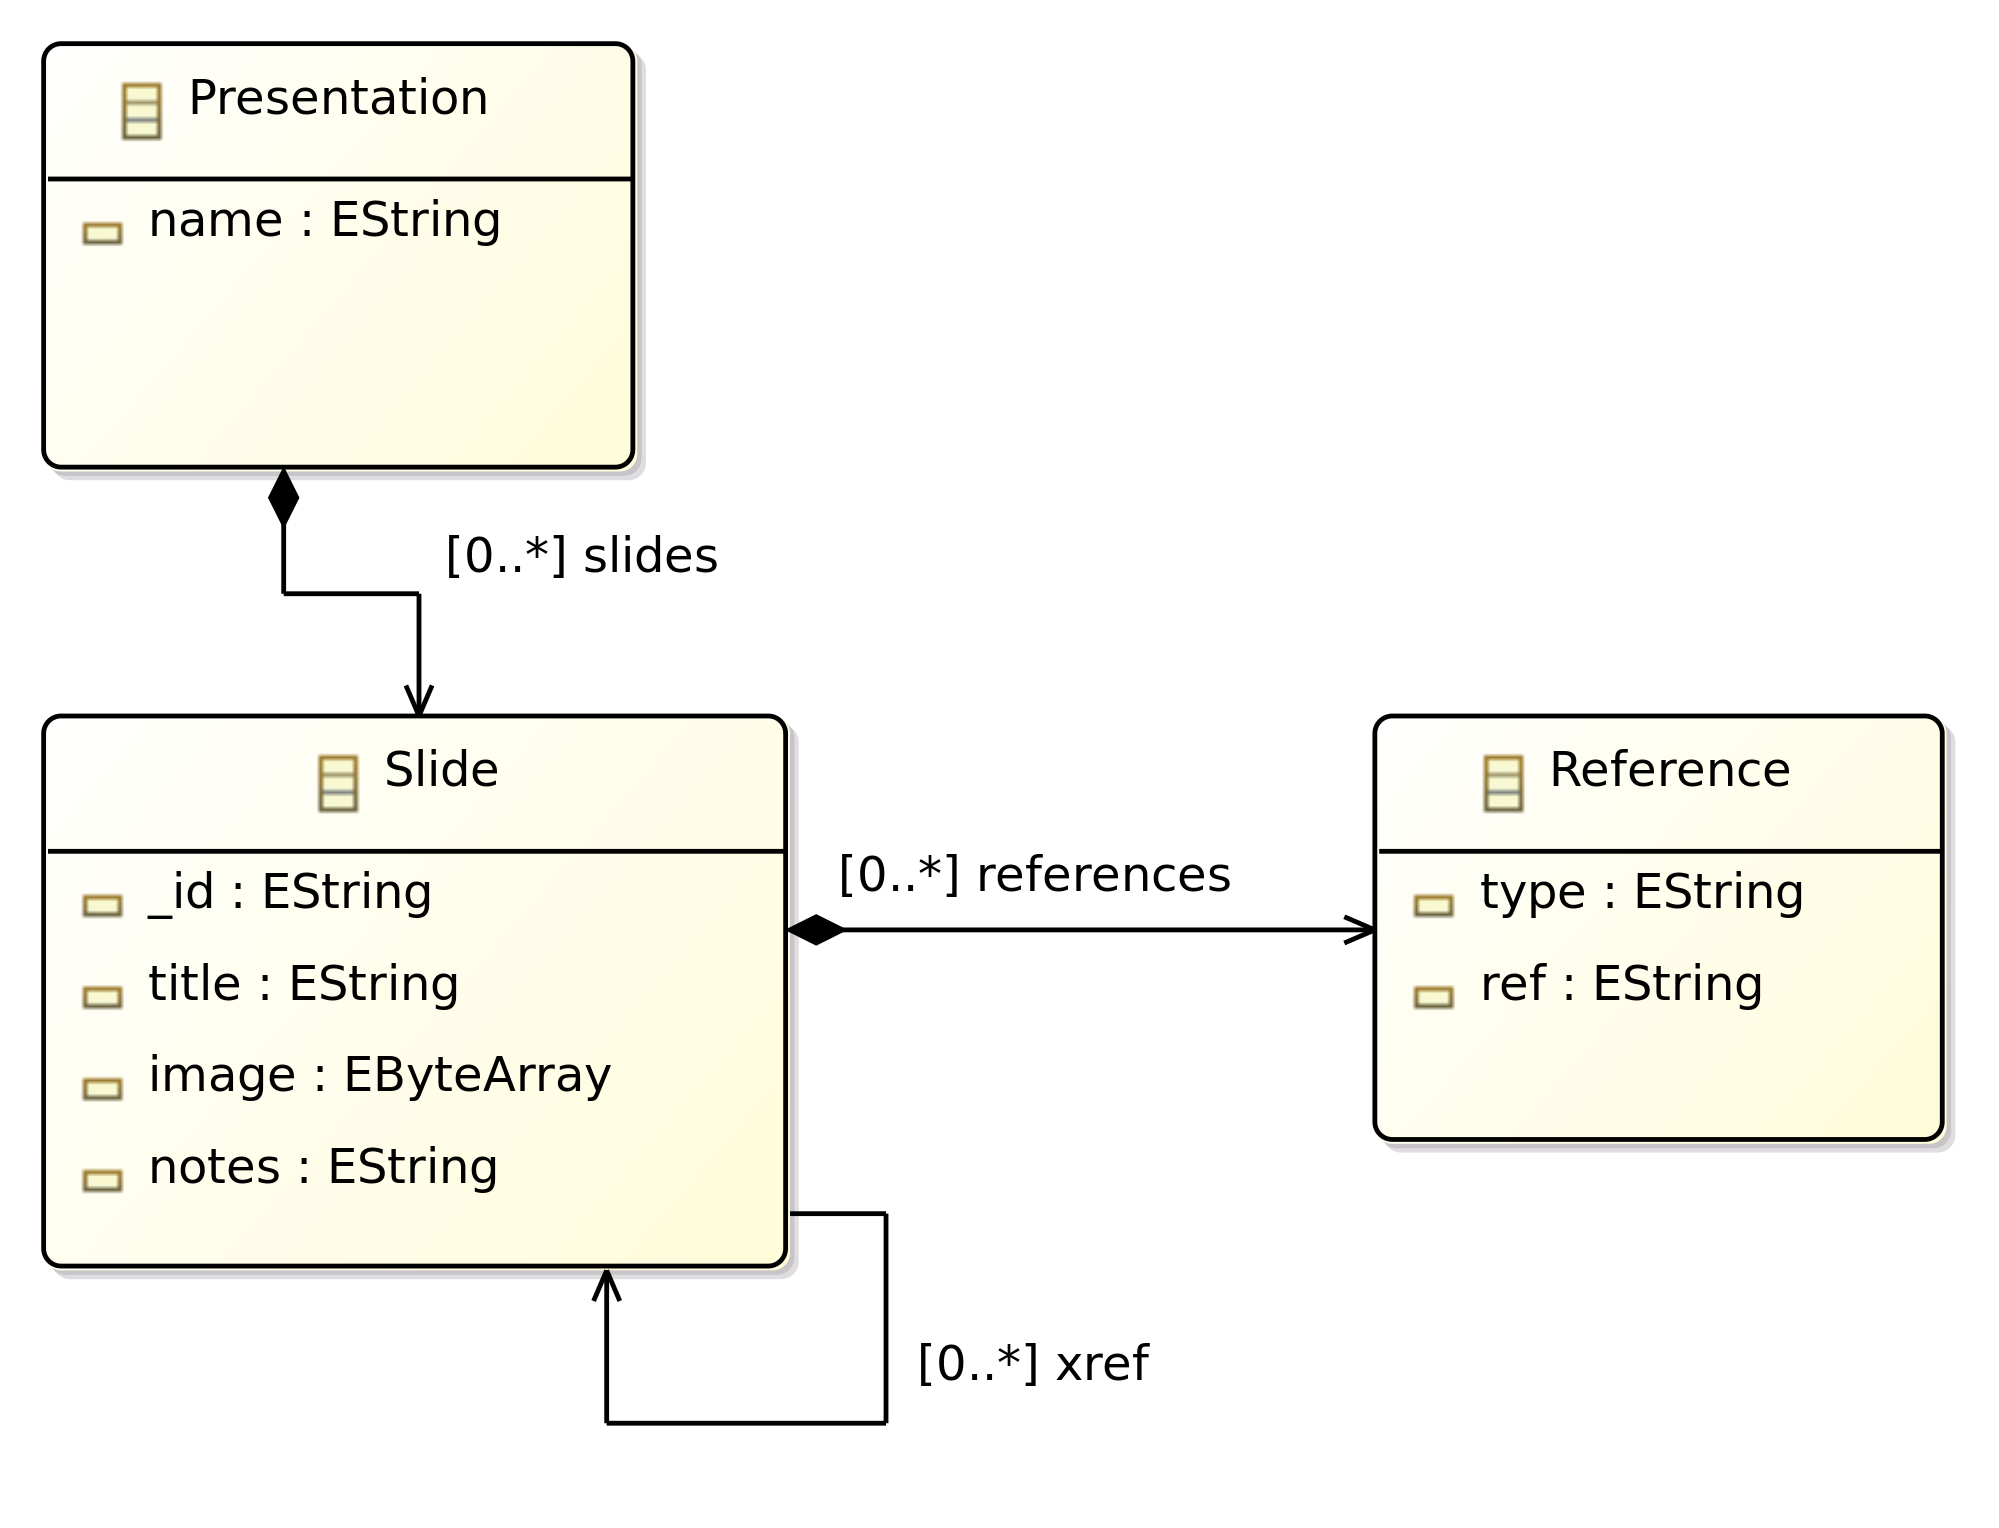
\includegraphics[width=.9\textwidth]{img/slides-data-model}

\framebreak

\begin{itemize}
\item OK, pensemos en {\bf relacional}
  \begin{itemize}
  \item \lstinline[language=sql]{CREATE TABLE ...}
  \item ¿Cuántas tablas?
  \item Claves ajenas, restricciones de integridad...
  \item {\bf Gap semántico}:
    \begin{itemize}
    \item La tabla {\tt Reference} no está contenida {\bf sino enlazada}
      (por clave ajena)
    \item O bien se crea la tabla {\tt Slide\_Reference}
    \item {\bf ID Artificial} para referencias
    \item Se tiene que crear la tabla {\tt Slide\_xref}
    \end{itemize}
  \end{itemize}

\end{itemize}

\begin{block}{El modelo de documentos es {\bf más natural en este caso}}
\end{block}

\framebreak

\begin{alertblock}{¿Y toda la información de diapositiva?}
\begin{itemize}
\begin{lstlisting}[language=sql]
SELECT * FROM Slides WHERE `_id` = 'slide000';
\end{lstlisting}
  \item ¿{\tt xref}? ¿{\tt references}?
\begin{lstlisting}[language=sql]
SELECT * FROM Jisbd17 s
  JOIN References r ON `s._id` = r.slide_id
  JOIN Slide_xref x ON `s._id` = x.slide_id
WHERE `s._id` = 'slide000';
\end{lstlisting}
\item Filas con {\bf ¡¡información replicada!!}
\item ¿Y si se añade más información a {\tt Slide}?
  \end{itemize}
\end{alertblock}

\framebreak

\begin{block}{MongoDB}
\begin{lstlisting}[language=Python]
slide = jisbd17.find_one({'_id': 'slide000'})
\end{lstlisting}
\end{block}

\end{frame}


\section{Introducción a los sistemas NoSQL}

\begin{frame}
  \frametitle{Introducción a NoSQL}
\begin{itemize}
% \item Sobre los \~{}2010s, se renueva la búsqueda de la escalabilidad, con
%   el abaratamiento del {\em hardware}
% \item Se {\bf diversifican los problemas}, la inclusión del {\bf análisis
%     de todos los datos disponibles por parte de las empresas}
% \begin{itemize}
% \item incluso de algunos que no se había pensado usar, p. ej. {\em
%     clickstreams\/}), {\bf publicidad a la carta}, etc.
% \end{itemize}
\item {\bf NoSQL} \ra{} {\em hashtag\/} llamativo que se
  eligió para una conferencia en~2009 (Johan Oskarsson de Last.fm)
\item Ahora se asocia a cientos de bases de datos diferentes,
  que se han clasificado en varios tipos (las veremos después),
  caracterizadas por {\bf no usar SQL} como modelo de datos
\item {\bf NoSQL} \ra{} {\bfseries\itshape Not Only SQL} (no sólo SQL)
% \item Big Data \ra{} hay una variedad de fuentes de datos ({\bf persistencia
%     polígota})
  \end{itemize}
\end{frame}

\begin{frame}[allowframebreaks]
  \frametitle{NoSQL -- ¿Por qué se plantearon?}
%En general, el desarrollo de NoSQL ha venido motivado, entre otras, por una
%serie de circunstancias:
\begin{enumerate}
\item {\bf Mayor escalabilidad horizontal}
  \begin{itemize}
  \item conjuntos de datos muy muy grandes
  \item sistemas de alto volumen de escrituras ({\em streaming\/} de
    eventos, aplicaciones sociales)
  \end{itemize}
\item {\bf Demanda de productos de software libre} (crecimiento de las {\em
    start-ups})
\item {\bf Consultas especializadas} no eficientes en el modelo relacional
  (JOINs)
\item {\bf Expresividad, flexibilidad, dinamismo}. Frustración con {\bf
    restricciones} del modelo relacional
  % \ra{} ({\bfseries\itshape schemaless})
%\item Paradigma {\bf funcional}: {\em Map-Reduce}
\end{enumerate}

\framebreak

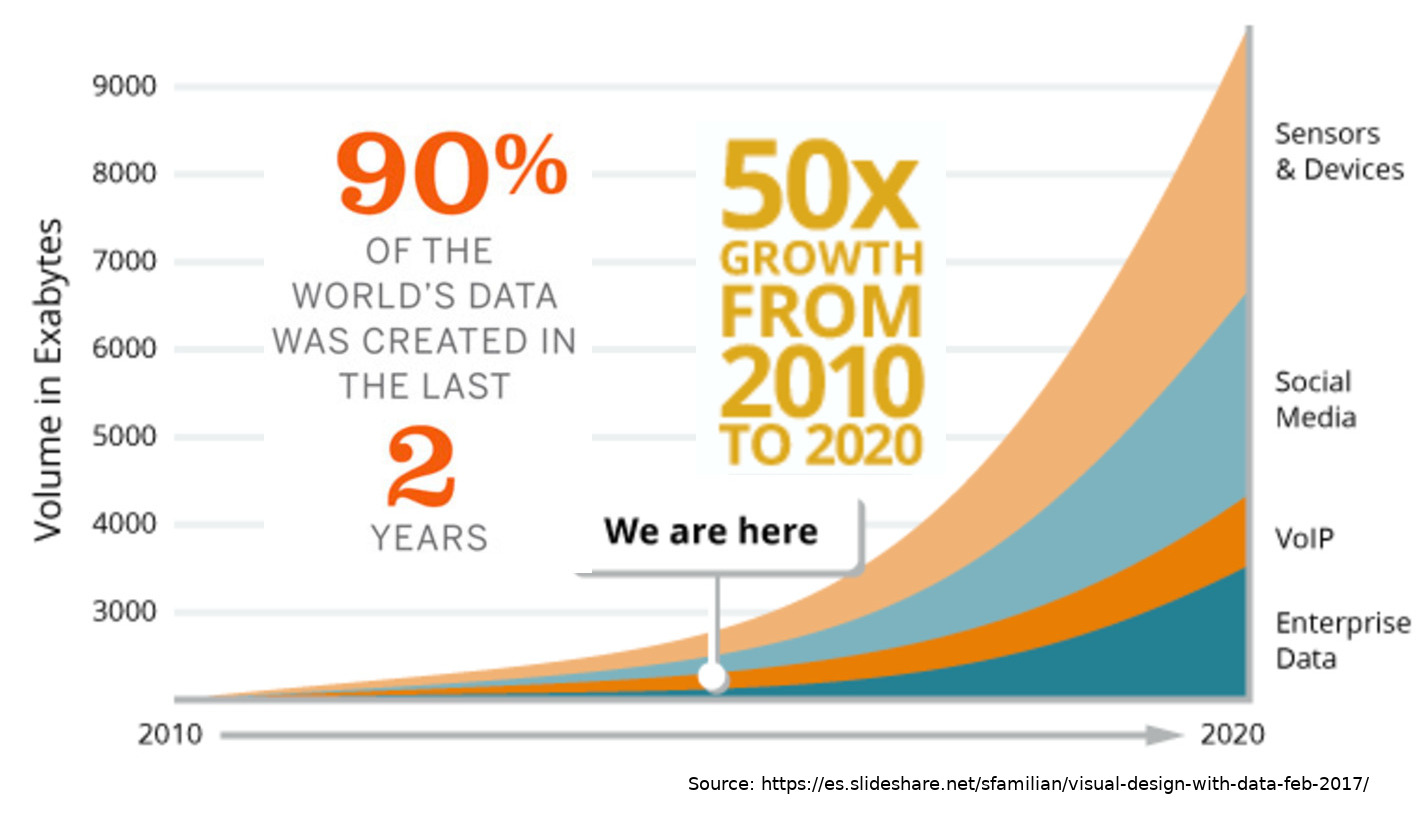
\includegraphics[width=\textwidth]{img/data-growth}

\end{frame}


\begin{frame}[allowframebreaks]
 \frametitle{NoSQL: Características}
\begin{itemize}
\item No se basan en SQL
\item Modelos de datos más ricos
\item Orientadas a la {\bf Escalabilidad}
\item Generalmente no obligan a definir un esquema \ra{}
  {\itshape\bfseries Schemaless}
\item Surgidos de la comunidad para solucionar problemas, y muchas de
  ellas son {\bf libres/{\itshape open source}}
\item Diseño basado en {\bf procesamiento distribuido}
\item Principios funcionales \ra{} {\bf MapReduce}
\end{itemize}

\framebreak

\begin{block}{Categorías de NoSQL}
    \begin{itemize}
    \item Bases de datos Key-Value
    \item Bases de datos Documentales
    \item Bases de datos columnares
    \item Bases de datos de grafos
    \item Bases de datos de arrays
    \end{itemize}
\end{block}
\end{frame}


\begin{frame}
  \frametitle{Evolución desde el modelo relacional}
\begin{itemize}
\item El {\bf modelo relacional} $\Rightarrow$ {\bf predominante en los
  últimos~\~{}30~años}
\item Tiene sus raíces en el denominado {\em business data processing},
  procesamiento de transacciones y {\em batch}
\item Propuesto por Codd en los~70, {\bf de alto nivel}
\item Actualmente los {\bf sistemas SQL están muy optimizados}:
\begin{itemize}
\item el {\bf grado de implantación es mayoritario}
\item para el 99\% de los problemas (que caben en un ordenador) es
  eficiente y adecuado
\end{itemize}
\end{itemize}
\end{frame}

% http://db-engines.com/en/ranking/


\begin{frame}
  \frametitle{Adopción de NoSQL}
Twitter cambiando a Cassandra por~2010\\
Cassandra desarrollada en Facebook en~2009\\
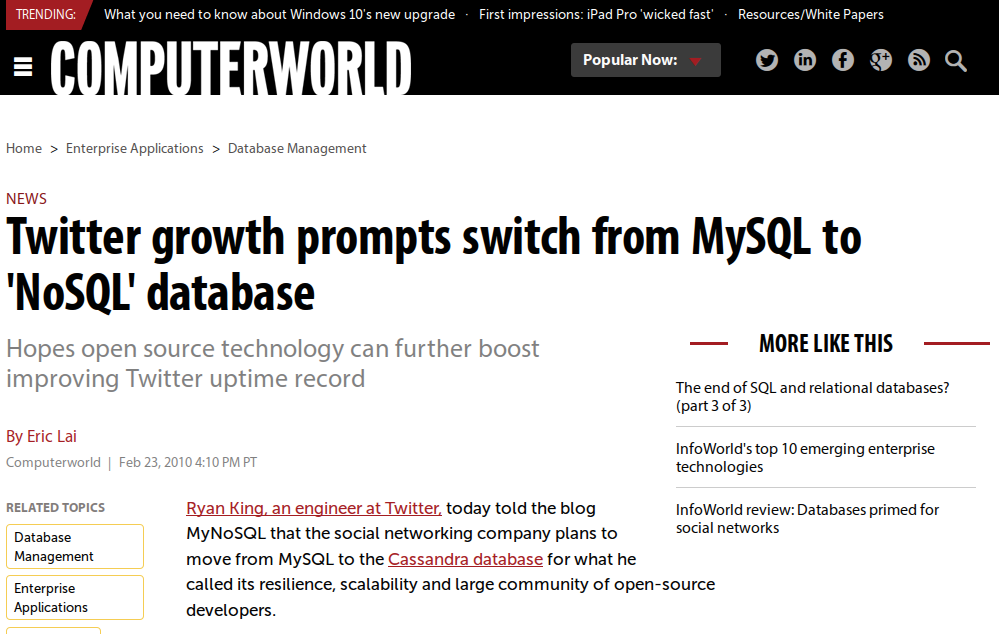
\includegraphics[width=\textwidth]{img/twitter-cassandra}
\end{frame}

\begin{frame}
  \frametitle{Adopción NoSQL. Ranking julio 2017}
\framesubtitle{Fuente: \url{http://db-engines.com/en/ranking/}}
\vspace*{.1ex}
\centering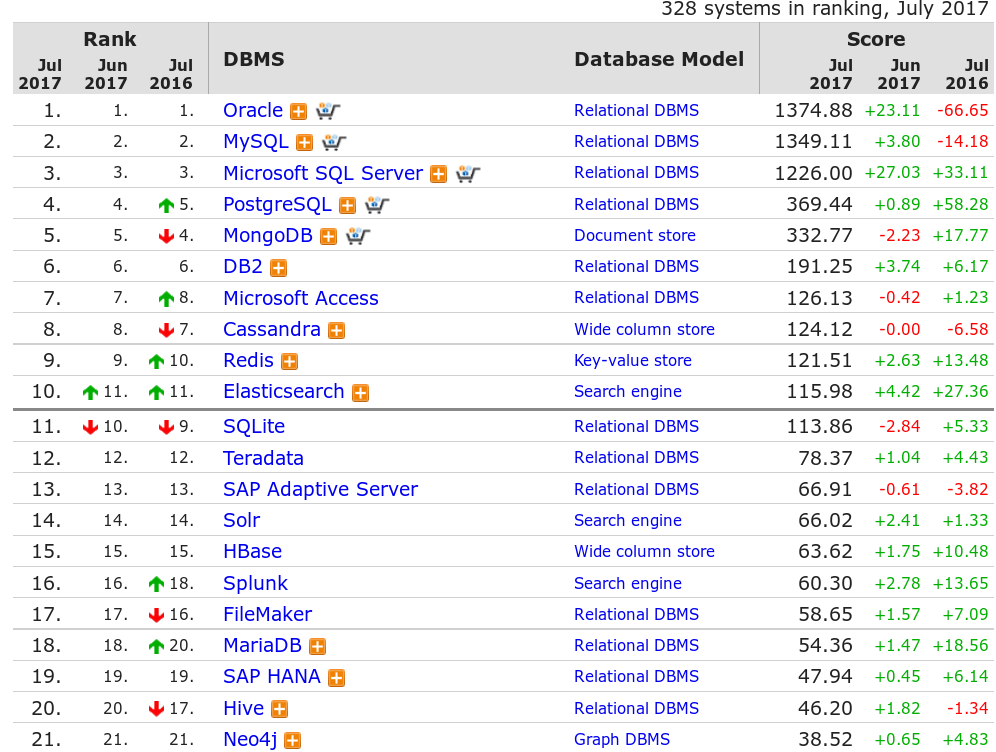
\includegraphics[width=.8\textwidth]{img/ranking-bbdd}
\end{frame}

\begin{frame}
\frametitle{Adopción NoSQL.Tendencia julio 2017}
\framesubtitle{Fuente: \url{http://db-engines.com/en/ranking/}}
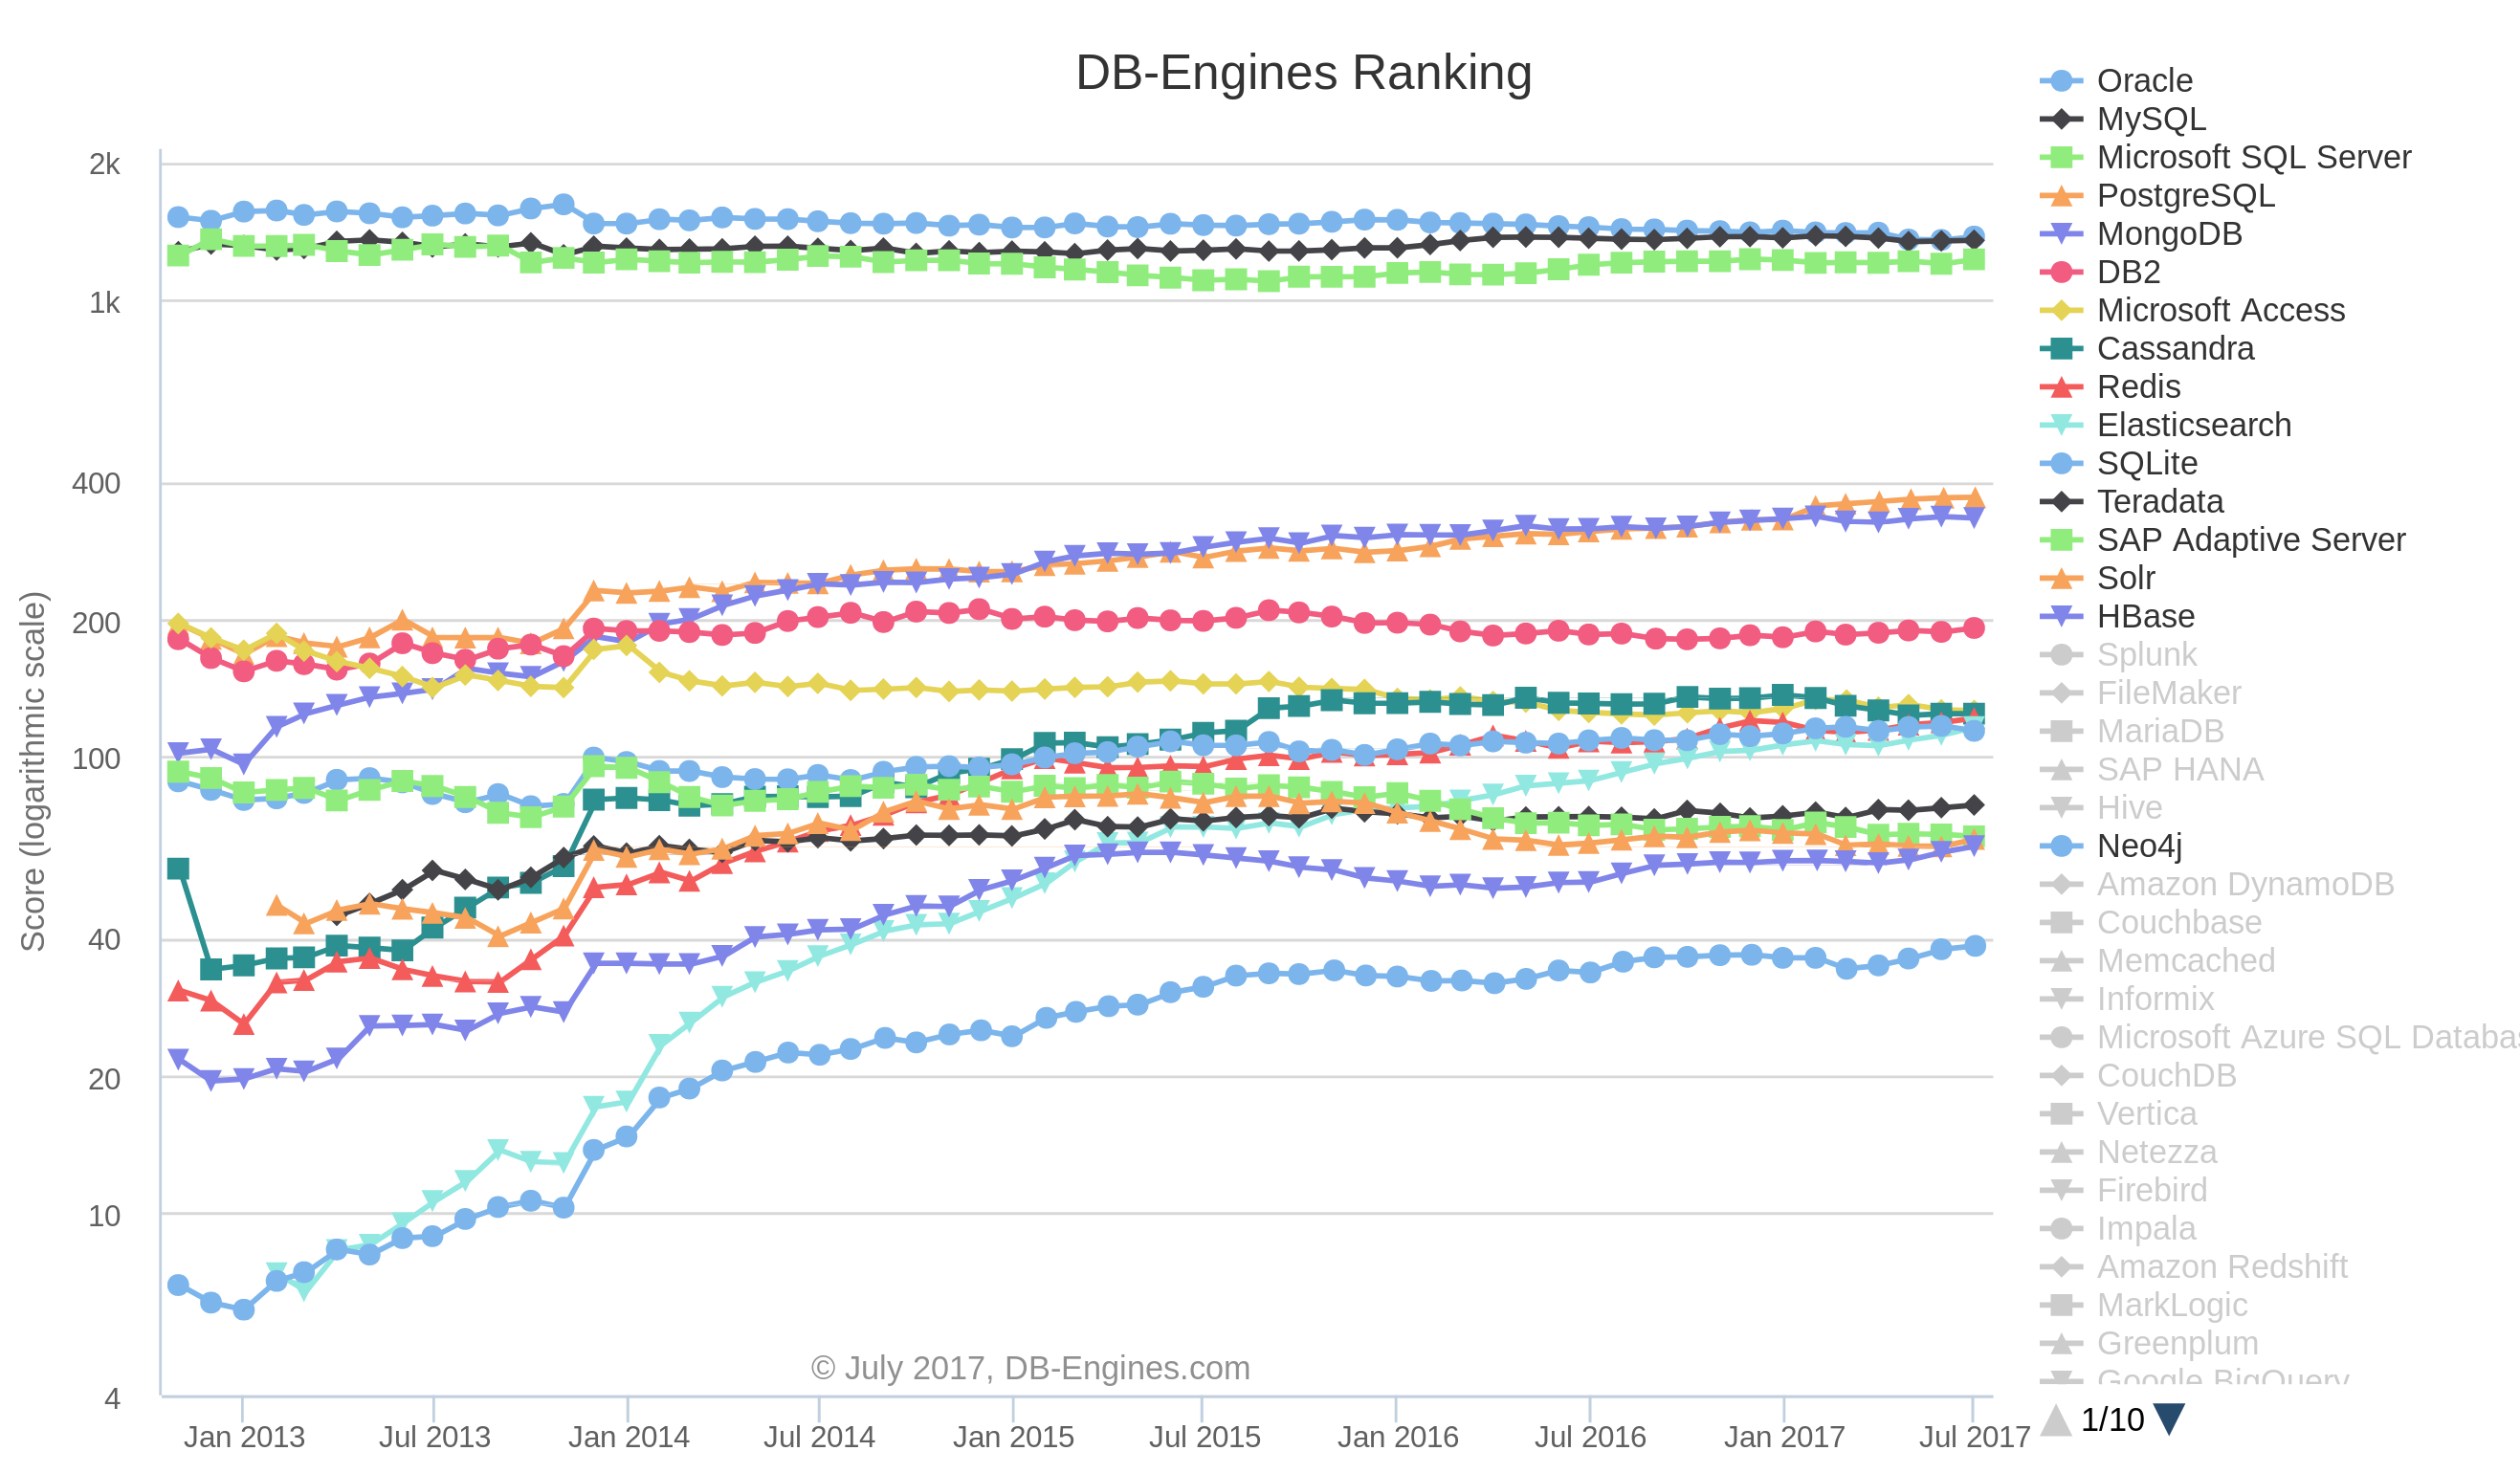
\includegraphics[width=\textwidth]{img/nosql-database-ranking}
\end{frame}

\begin{frame}
  \frametitle{Adopción NoSQL. Análisis}
\begin{alertblock}{Análisis}
\begin{itemize}
\item Dominan los grandes SGBDR
\item El {\em Open Source} tiene una importancia crucial (MySQL,
  MongoDB, etc.)
\item Varias bases de datos NoSQL entre las~10 primeras. Muchas en las~20
  primeras
\item La distancia entre los grandes SGBDR y el primer NoSQL (MongoDB) es
  de~5$\times$
\item Paradigmas más ``atrevidos'' como el de grafos están entre los~20
  primeros (Neo4j)
\end{itemize}
  \end{alertblock}
\end{frame}



\subsection{La importancia de la escalabilidad}

\pgfdeclareimage[height=2.7em]{sobremesa}{img/server1}%img/servidor}
\pgfdeclareimage[height=.7em]{switch}{img/switch1}%img/switch}

\newsavebox{\network}

\begin{lrbox}{\network}
\begin{tikzpicture}
  \foreach \x in {0,...,5}
    \foreach \y in {0,...,3}
    \node [] (\x\y) at (1.5*\x,1.5*\y) {\pgfuseimage{sobremesa}};

% switch
\node[inner sep=0pt] (switch) at (1.5*2.5, 1.5*4) {\pgfuseimage{switch}};

\begin{scope}[on background layer]
  \foreach \x in {0,...,5}
    \foreach \y in {0,...,3}
      \draw[gray!50] (switch)--(\x\y) ;
\end{scope}
\end{tikzpicture}
\end{lrbox}

\begin{frame}
\frametitle{Cambio de perspectiva: Red}

\begin{overlayarea}{\textwidth}{.8\textheight}
\only<1->{%
\begin{center}
\usebox{\network}
\end{center}%
}%
\only<2>{
\vspace*{-13em}
  \begin{block}{Almacenamiento distribuido}
    \begin{itemize}
    \item Desde los 90's: Clústers/NOC/COW: procesamiento masivamente
      paralelo
\begin{center}
{\color{red}SIN EMBARGO...}
\end{center}
\item Almacenamiento no distribuido
\item Ahora los nodos $\Rightarrow$ también {\bf almacenamiento}
\item Minimizar el verdadero cuello de botella: {\bf trasiego de
    información por la red}
    \end{itemize}

  \end{block}%
}%
\only<3>{
\vspace*{-10em}
\begin{block}{Procesamiento distribuido}
\begin{itemize}
\item Necesidad de {\bf paralelización máxima}
\item {\bf Escalabilidad}
\item Explotación de la {\bf localidad de los datos}:
  \begin{itemize}
  \item Datos producidos se utilizan en siguientes iteraciones
\item Datos recibidos directamente (clientes simultáneos)
\end{itemize}
\end{itemize}
\end{block}
}%
\only<4>{
\vspace*{-9em}
\begin{block}{Procesamiento distribuido}
\begin{itemize}
\item Vuelta al modelo funcional inherentemente paralelo: (i.e. {\bf
    Map-Reduce})
\item Almacenamiento distribuido: (i.e. {\bf HDFS})
\item Coordinación distribuida: (i.e. {\bf Zookeeper})
\end{itemize}
\end{block}%
}%
\only<5>{
\vspace*{-13em}
\begin{block}{Modelo de datos}
\begin{itemize}
  \item El modelo relacional limita a tablas con valores primitivos y
    relaciones {\em Primary Key\/}/{\em Foreign Key}
  \item Pero en programación se utilizan {\bf listas}, {\bf arrays}, {\bf
      tipos de datos compuestos} ({\color{red}{\em gap\/} semántico})
  \item ACID es {\bf muy compleja y costosa} en ambientes distribuidos
    (quizá {\bf no necesaria} en algunas aplicaciones)
\end{itemize}
\end{block}%
}%
\only<6>{
\vspace*{-11em}
\begin{block}{Modelo de datos (ii)}
\begin{itemize}
\item ¿Si se pudiera ver como un {\bf GRAN ARRAY}?
\begin{itemize}
\item Cada nodo almacenaría una parte del array
\item Búsqueda aleatoria {\bf muy rápida} (árboles B)
\item Uso de {\bf filtros de Bloom}
\item Uso de {\bf objetos complejos} (p. ej. {\bf documentos JSON}),
  para mantener la {\bf localidad espacial de datos relacionados} (+
  después)
\item Transacciones limitadas al {\bf objeto complejo}
\end{itemize}
\end{itemize}
\end{block}%
}%
\end{overlayarea}
\end{frame}

\subsection{Schemaless}

\begin{frame}[fragile,allowframebreaks]
  \frametitle{Schemaless}
\begin{itemize}
\item NoSQL (en general) {\bf no requiere de un esquema}
\begin{alertblock}{}
  \centering
  \href{https://farm6.staticflickr.com/5483/29931060254_109e3e36da_o_d.jpg}{\bf
    SCHEMALESS}
\end{alertblock}
\item {\bf Flexibilidad}: Posibilidad de almacenar documentos con una
  estructura diferente
\begin{itemize}
\item Tratar información incompleta
\item Evolucionar la base de datos/esquema
\item Añadir nuevas características a las aplicaciones
\end{itemize}
\end{itemize}

\framebreak

\begin{small}
\begin{tabular}{p{.43\textwidth}cp{.43\textwidth}}
{\bfseries\itshape schema-on-write}&$\Rightarrow$&{\bfseries\itshape
                                                   schema-on-read}\\
\midrule
\rowcolor{blue!20} SQL&&NoSQL\\
\rowcolor{blue!15} Los datos conforman cuando se {\bf escriben}&&Los datos leídos conforman a
                                               un {\bf esquema implícito}\\
\rowcolor{blue!20} {\bf Tipado estricto} (estático) && {\bfseries\itshape Duck-Typing}
                                    (dinámico) \\
\rowcolor{blue!15}  Datos homogéneos && Datos {\bf heterogéneos}\\
\rowcolor{blue!20} Proceso analítico a través de {\bf consultas} && {\bfseries\itshape Use as read}\\
\end{tabular}
\end{small}
% \item Se pasa de {\em schema-on-write} (se asegura que los
%   datos son conformes cuando se escriben, como en relacional) a {\em
%     schema-on-read} (los datos tienen un {\bfseries\itshape esquema
%     implícito} cuando se leen)
% \item Así, las bases de datos NoSQL están más cerca de los lenguajes
%   dinámicos, mientras que las relacionales más cerca de los lenguajes
%   estáticos
% \end{itemize}

\framebreak

\begin{itemize}
\item {\bf Ejemplo}: Añadir el campo {\tt first\_name} a partir del campo
  {\tt name}
\item Los nuevos objetos se crean con el nuevo formato
\item A la hora de leerlos, se puede hacer:
\end{itemize}
\begin{lstlisting}
if (user && user.name && !user.first_name) {
   // Docs anteriores a 2013 no tienen first_name
   user.first_name = user.name.split(" ")[0];
}
\end{lstlisting}

\framebreak

\begin{itemize}
\item En SQL puede ser un proceso muy costoso (procesa toda la tabla, {\em
    locking\/}, puede que haya que parar las aplicaciones):
\end{itemize}
\begin{lstlisting}[language=SQL]
ALTER TABLE users ADD COLUMN first_name text;
UPDATE users SET first_name =
    substring_index(name, ' ', 1);
\end{lstlisting}

\framebreak

\begin{block}{¿Cuándo es apropiado {\em schemaless}?}
  \begin{itemize}
  \item {\bf Objetos heterogéneos}
\item Estructura de los datos {\bf impuesta externamente}
\item Si intuimos que los datos {\bf cambiarán en el futuro}
  \end{itemize}
\end{block}


\framebreak

\begin{block}{SIN EMBARGO...}
 A veces {\bf un esquema es conveniente}
\begin{itemize}
\item Facilita el desarrollo y evita inconsistencias
  \begin{itemize}
  \item {\tt Mongoose} para MongoDB:
  \end{itemize}
\end{itemize}
\begin{lstlisting}[language=Java]
var Comment = new Schema({
  name: { type: String, default: 'Anonymous' },
  date: { type: Date, default: Date.now },
  text: Buffer
});
// a setter with on-line modification
Comment.path('name').set(function (v) {
  return capitalize(v);
});
\end{lstlisting}
\end{block}
\end{frame}


\begin{frame}
  \frametitle{Choose wisely}
\begin{columns}
\begin{column}{.5\textwidth}
  
\includegraphics[height=.7\textheight]{img/chose-wisely}
\end{column}
\begin{column}{.5\textwidth}
\begin{alertblock}{SQL}
\end{alertblock}
\begin{alertblock}{NoSQL}
\end{alertblock}
\begin{alertblock}{Polyglot Persistence}
\end{alertblock}
\end{column}
\end{columns}
\end{frame}


\subsection{Modelado de datos en NoSQL}

\begin{frame}[allowframebreaks]
  \frametitle{Modelado de datos en NoSQL}
El modelado de datos debe ser:
  \begin{itemize}
  \item Realizado al mayor nivel de abstracción posible
  \item Independiente de la tecnología subyacente
  \end{itemize}
Sin embargo, en NoSQL:
  \begin{itemize}
  \item Se tiene que tener en cuenta el diseño {\bf distribuido}
  \item {\bf Optimización guiada por las consultas}
  \end{itemize}

  \framebreak
Con respecto al modelo de datos:

\begin{itemize}
\item Se mantienen los conceptos de entidad, relación, cardinalidades, etc.
\item El modelado relacional se centra en especificar {\bf qué datos
    tenemos y podemos ofrecer}
\item El modelo NoSQL se centra en {\bf optimizar qué
    consultas vamos a servir}
\item Es ``barato'' {\bf duplicar (desnormalizar)} los datos si con ello se
  consigue {\bf mayor eficiencia de acceso}
\end{itemize}

\end{frame}

\begin{frame}
  \frametitle{Representación relacional de un CV}
\framesubtitle{Kleppmann, 2016. \emph{Designing Data Intensive Applications}}
  \centering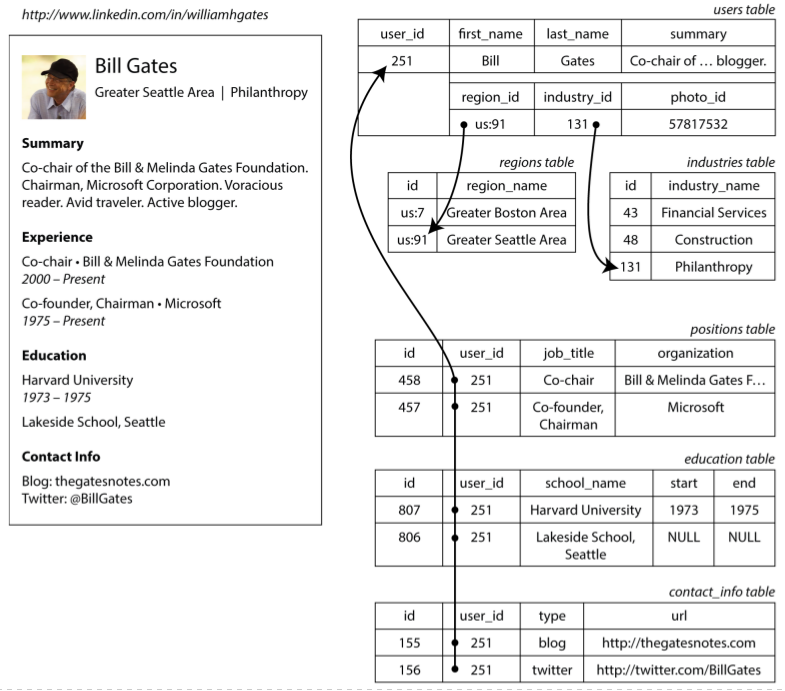
\includegraphics[height=.81\textheight]{img/gates}
\end{frame}

\begin{frame}
  \frametitle{Representación de relaciones}
  \framesubtitle{Relaciones uno a muchos}

  Las relaciones uno a muchos (e.g. {\tt positions}) en el modelo
  relacional:

\begin{itemize}
\item Normalización usando varias tablas ({\tt Positions} con
  {\tt user\_id})
  \begin{itemize}
  \item Necesidad de más de una tabla
  \item Necesidad de uso de {\tt JOIN} $\Rightarrow$ ineficiencia
  \end{itemize}
\item Algunos SGBDR ofrecen la posibilidad de tener tipos de datos
  estructurados y campos XML o JSON. (P. ej. PostgreSQL)
  \begin{itemize}
  \item Alternativa interesante, aunque...
  \item No son estándar
  \end{itemize}
\end{itemize}
\end{frame}

\begin{frame}[plain,fragile]
%  \frametitle{CV como un documento}
\begin{lstlisting}[language=json,basicstyle=\tiny\tt]
{
  "user_id": 251,
  "first_name": "Bill",
  "last_name": "Gates",
  "summary": "Co-chair of the Bill & Melinda Gates... Active blogger.",
  "region_id": "us:91",
  "industry_id": 131,
  "photo_url": "/p/7/000/253/05b/308dd6e.jpg",
  "positions": [
    {
      "job_title": "Co-chair",
      "organization": "Bill & Melinda Gates Foundation"
    },
    {
      "job_title": "Co-founder, Chairman",
      "organization": "Microsoft"
    }
  ],
  "education": [
    {
      "school_name": "Harvard University",
      "start": 1973,
      "end": 1975
    },
    {
      "school_name": "Lakeside School, Seattle",
      "start": null,
      "end": null
    }
  ],
  "contact_info": {
    "blog": "http://thegatesnotes.com",
    "twitter": "http://twitter.com/BillGates"
  }
}
\end{lstlisting}
\end{frame}

\begin{frame}
  \frametitle{CV como un árbol (equivalente)}
\centering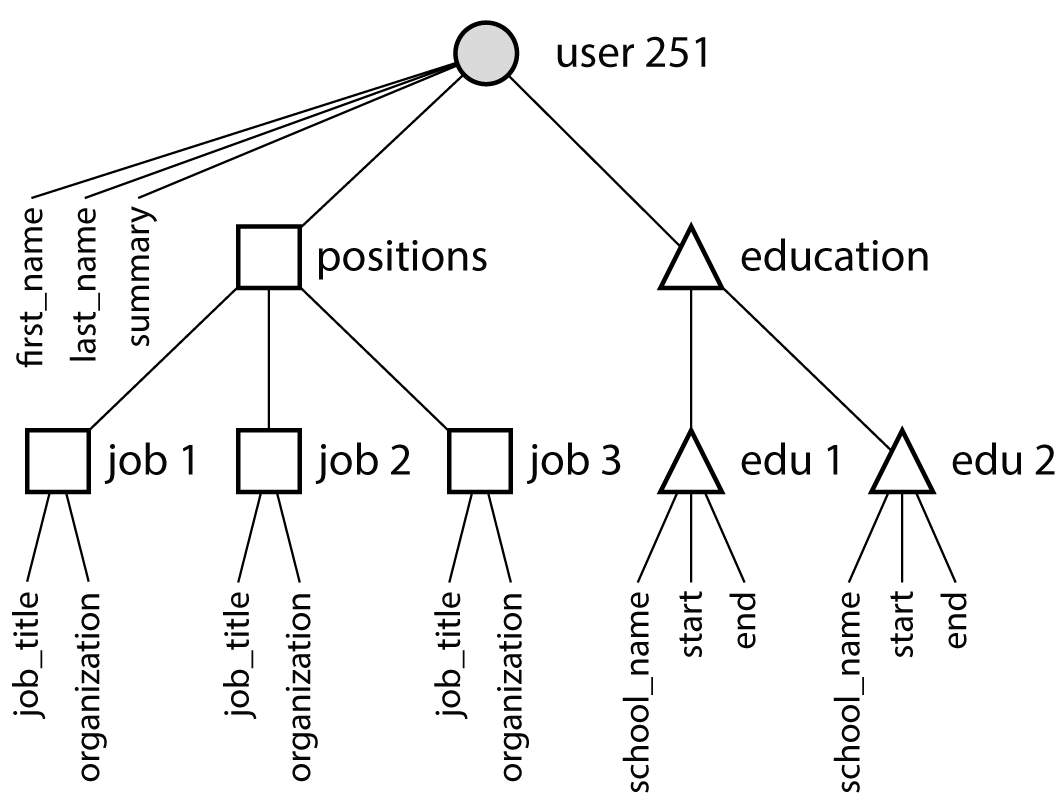
\includegraphics[height=.85\textheight]{img/tree}
\end{frame}

\begin{frame}[allowframebreaks]
  \frametitle{Representación de Relaciones}
\framesubtitle{Modelo de documentos}
\begin{itemize}
\item {\bf Modelo de documentos} \ra{} analogía del {\bf array/mapa
    gigante}
\item {\bf Conjunto de documentos} (objetos complejos)
  \begin{itemize}
\item Un {\bf identificador único}, campo {\em id\/}
\item Búsqueda aleatoria eficiente por clave ({\bf referencia})
\item Estructura jerárquica de sub-documentos contenidos \ra{}
  {\bf agregación}
\end{itemize}
\end{itemize}


\begin{alertblock}{}
  Más flexibilidad que el modelo relacional (elección entre \underline{\em
    referencia} y \underline{\em agregación})
\end{alertblock}

\end{frame}

\begin{frame}[allowframebreaks]
  \frametitle{Representación de Relaciones}
\framesubtitle{Uno a muchos (ii) -- NoSQL}
\begin{itemize}
\item Relaciones {\bf Uno a Muchos} ({\tt positions}):
  \begin{itemize}
  \item {\bf Opción 1}: Agregando la tabla {\tt positions}
  \item {\bf Opción 2}: Convertir las empresas en entidades, y utilizar una
    {\bfseries\itshape referencia}
  \end{itemize}
\item ¿Qué opción elegir?
\end{itemize}

\framebreak

\begin{alertblock}{¡Modelo guiado por el acceso a datos!}
\begin{small}
  \begin{itemize}
  \item Si los elementos ``muchos'' tienen una estructura sencilla
    \ra{} {\bf Opción~1}
\item Si los elementos ``muchos'' son usualmente {\bf recuperados en una
    consulta} junto con el elemento ``uno'' \ra{} {\bf Opción~1}
\item Si los elementos ``muchos'' son relativamente grandes, o bien son
  recuperados siempre de forma separada \ra{} {\bf Opción~2}
  \end{itemize}
\end{small}
\end{alertblock}
\end{frame}

\begin{frame}
  \frametitle{Representación de Relaciones}
  \framesubtitle{Muchos a uno y muchos a muchos}
Relaciones muchos a uno y muchos a muchos:
    \begin{itemize}
    \item Personas que viven en una región
\item Preguntas que refieren a Tags
    \end{itemize}
El modelo de documentos no aporta ventajas
  \begin{itemize}
  \item La {\em agregación} daría lugar a mucha {\bf duplicación} (y a
  problemas de sincronización)

\item {\color{red} $\Rightarrow$} {\bf Referencias} (sobre el ID), similar
  a una FK en el modelo relacional
\begin{itemize}
  \item {\color{red} $\Rightarrow$} al no haber {\bf JOINs} la aplicación
    tiene que hacer más de una petición a la BD
  \end{itemize}
\end{itemize}
\end{frame}

\begin{frame}
  \frametitle{Muchos a muchos -- referencia}
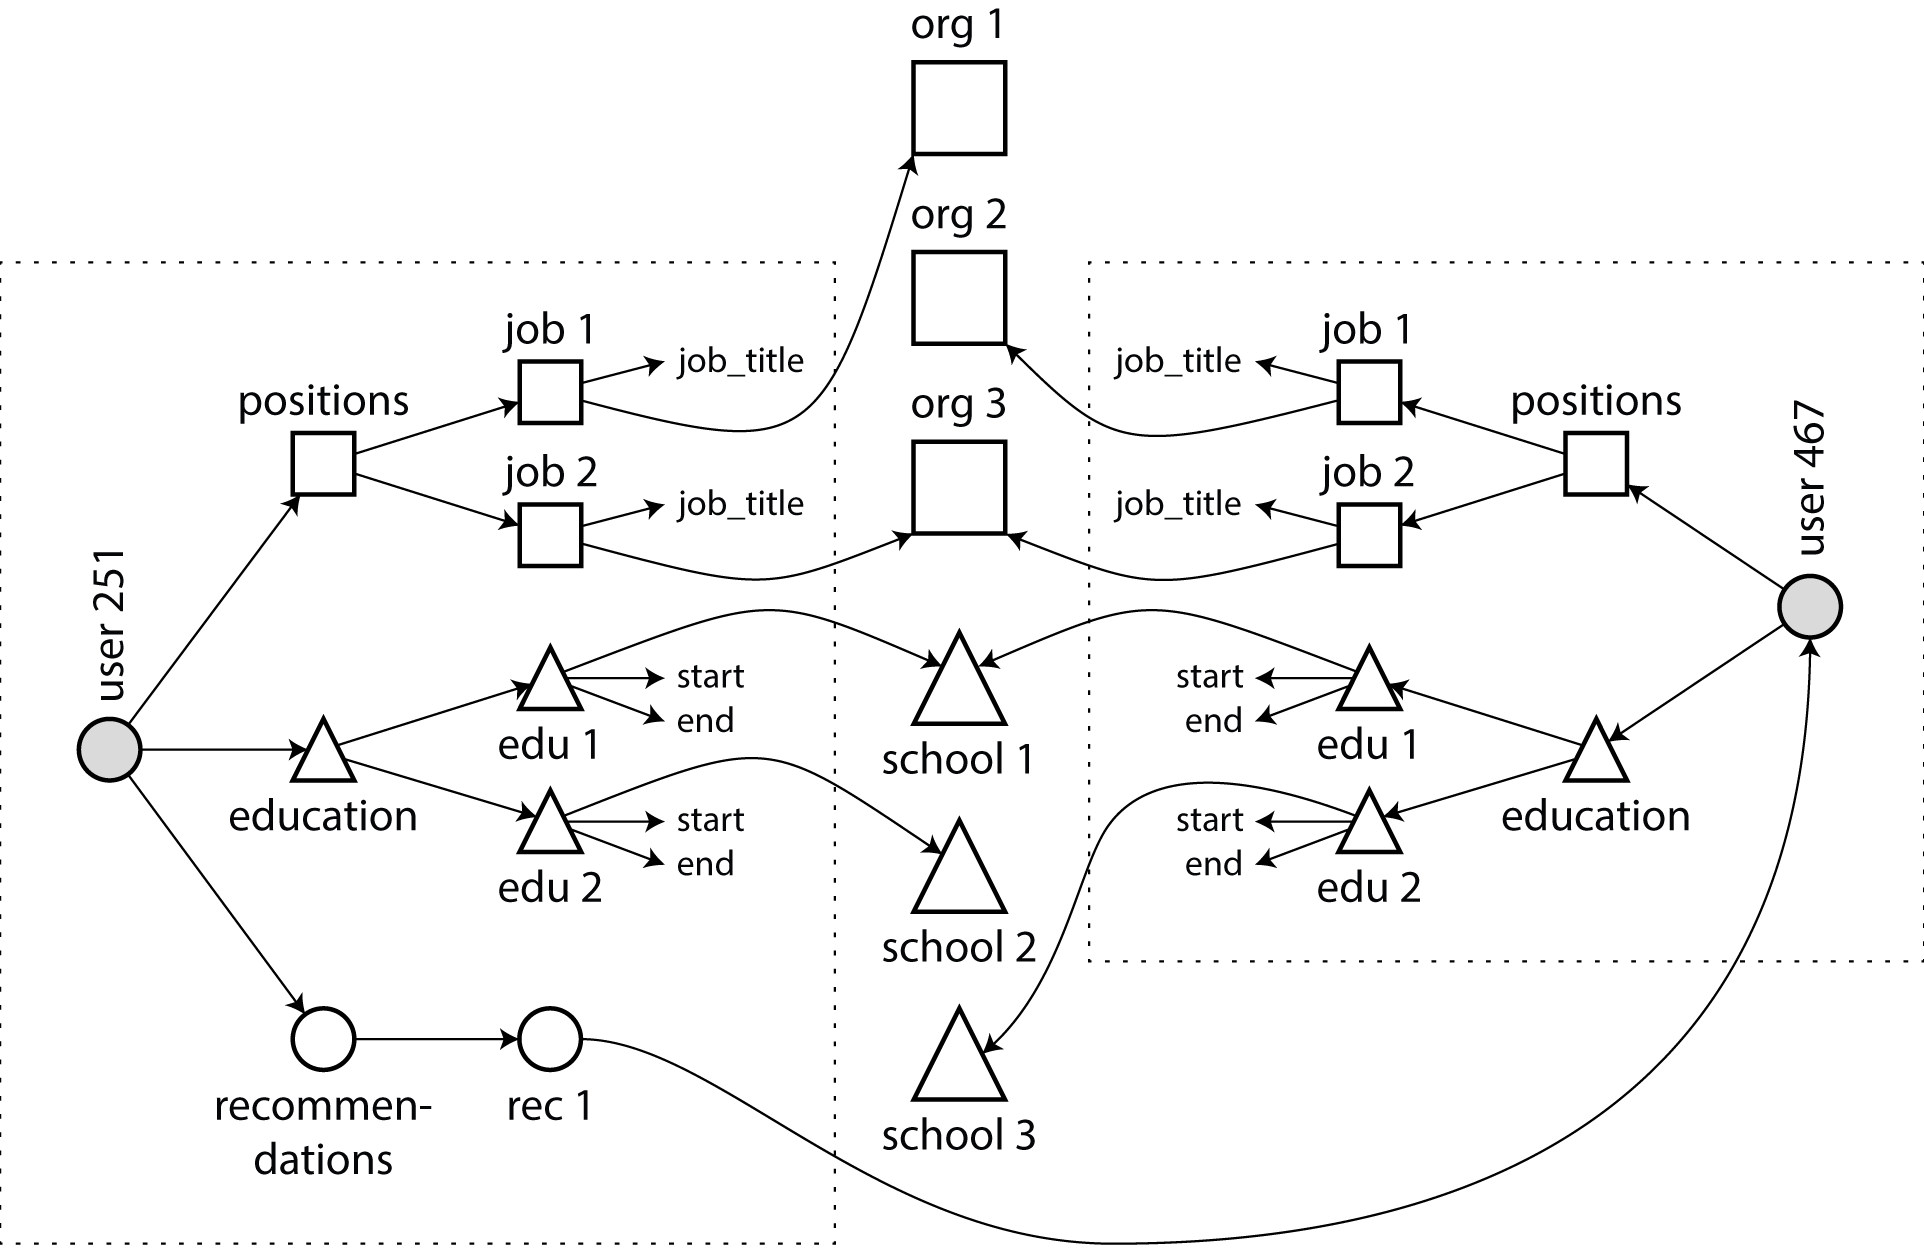
\includegraphics[width=\textwidth]{img/many-to-many}
\end{frame}

% \begin{frame}
%   \frametitle{Reconsiderando el modelo de documentos}
%   \begin{itemize}
%   \item Las ventajas del modelo basado en documentos son:
%     \begin{itemize}
%     \item Para algunas aplicaciones, la abstracción de documentos se acerca
%       más al modelo de datos
% \item La abstracción de documentos aporta más flexibilidad al esquema. Por
%   ejemplo, se pueden añadir campos diferentes a cada documento (también
%   llamados modelos {\itshape\bfseries schemaless\/})
% \item En algunos casos puede mejorar la eficiencia gracias a la localidad
%   (agregación)
%     \end{itemize}
%   \end{itemize}
% \end{frame}


\subsection{Eficiencia {\em raw}}

\begin{frame}[allowframebreaks]
  \frametitle{Eficiencia {\em raw}}
  \begin{itemize}
  \item Los sistemas NoSQL tienen que competir también con los SQL en
    términos de eficiencia neta (también llamada {\em raw})
  \item Un pequeño test sintético nos puede ayudar a hacernos una
    idea\footnote{\url{http://bonesmoses.org/2016/07/15/pg-phriday-a-postgres-persepctive-on-mongodb/}.}

\item La prueba se realizó sobre MongoDB y sobre MySQL (se ha adaptado el
  original, que era para PostgreSQL)

  \framebreak

\item Se parte de una tabla sencilla con cuatro valores, que muestran
  medidas de sensores con localización, valor de la lectura y una marca de
  tiempo
  \item Se realizan seis pruebas que pueden corresponder a un conjunto de
    consultas normales:
  \framebreak
  \begin{enumerate}
  \item Inicialmente se insertan {\bf un millón} de elementos generados al
    azar, con fechas que permitan la búsqueda por rango ({\bf Fill})
  \item Se crea un índice en la tabla para la fecha de la lectura ({\bf
      Index})
  \item Se actualizan los valores de un conjunto de entradas seleccionadas
    por rango de fechas ({\bf Update})
  \item Se eliminan un conjunto de filas seleccionadas por rango de fechas
    ({\bf Delete})
  \item Obtiene el número de filas restantes ({\bf Count})
  \item Se obtiene un {\bf subconjunto} de filas extraído de una consulta
    dada por un rango de fechas ({\bf Interval})
  \end{enumerate}

\end{itemize}

\begin{center}
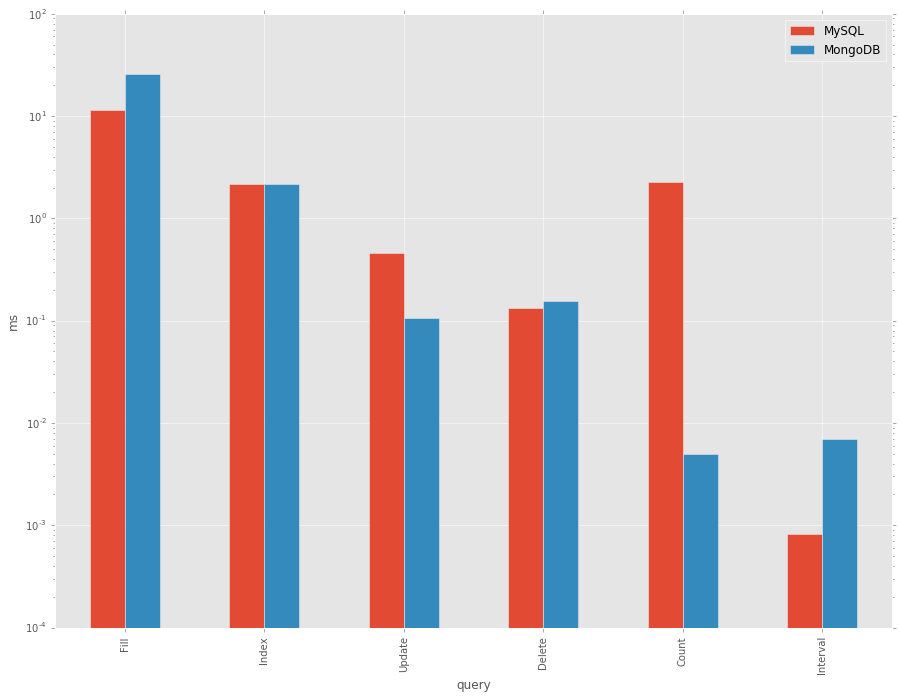
\includegraphics[width=.9\textwidth]{img/mongo_vs_mysql}
\end{center}


\begin{itemize}
\item El gráfico tiene escala logarítmica en el eje Y (las
  diferencias pequeñas se acentúan)
\item A simple vista, ambos están muy igualados
  \begin{itemize}
  \item SQL (MySQL) lleva {\em muchos años} de optimizaciones
  \item MongoDB tiene menos historia a sus espaldas en cuanto a
    optimizaciones, etc.
  \end{itemize}
\item Hay casos en los que uno es más rápido que el otro y viceversa

\framebreak

\item No se puede decir cuál es mejor
  \begin{itemize}
  \item {\bf \color{red} $\Rightarrow$ DEPENDE DEL PATRÓN DE ACCESOS QUE VAYA A
      TENER NUESTRA APLICACIÓN}
  \item (p. ej. contado en MongoDB mucho más rápido que en MySQL;
    actualización algo más rápida)
  \end{itemize}
\end{itemize}

\end{frame}

% \begin{frame}
%   \frametitle{Map-Reduce}
% \begin{itemize}
% \item La escalabilidad de las bases de datos relacionales está limitada por
%   la ley de Moore
% \item Los {\em clústers} surgieron como una alternativa para proporcionar
%   {\em escalabilidad horizontal} (vs. escalabilidad vertical, mejorar un
%   procesador)
% \item Sin embargo, las bases de datos relacionales no casan bien con los
%   clústers ({\em joins} en tablas muy grandes, tablas temporales, etc.)
% \item Como se ha dicho, las bases de datos NoSQL surgieron como una
%   respuesta a estas limitaciones
%   \begin{itemize}
%   \item Al preferir la {\bf agregación} (localidad) a la referencia (claves
%     ajenas), cada entidad almacenada se hace más independiente
% \item Por lo tanto, se puede almacenar de forma más sencilla en un {\em
%     pool} de servidores
% \item Se adoptó también el paradigma funcional de procesamiento de datos
%   $\Rightarrow$ {\bf Map-Reduce}
% \item Millones de máquinas ejecutan {\bf en paralelo procesos} sobre datos
%   que están {\bf físicamente distribuidos}, alojando los resultados {\bf
%     localmente en cada servidor} (descentralización, HDFS, Hadoop, etc.)
%   \end{itemize}
%   \end{itemize}
% \end{frame}

\section{Tipos de Sistemas NoSQL}


\subsection{Key-Value y Documentales}

\begin{frame}
  \frametitle{Key-Value Stores y Documentales}
  
\includegraphics[width=\textwidth]{img/MongoDB}
\end{frame}

\begin{frame}[allowframebreaks]
  \frametitle{Key-Value Stores y Documentales}
\vspace*{-.9em}
\begin{itemize}
\item A cada pieza de datos se le asigna un identificador
\item La diferencia entre ambas es que:
  \begin{itemize}
  \item En {\bf Key-Value}, el valor es opaco (es un {\em blob\/})
  \item En las documentales, la base de datos puede ver el contenido del
    agregado, y utilizar su información como parte de las búsquedas y
    actualizaciones
\end{itemize}
\item Documentos $\Rightarrow$ formatos jerárquicos tipo JSON o XML
\framebreak
\item La diferencia entre ambas un poco difusa
  \begin{itemize}
  \item Por ejemplo, Riak es Key-Value pero permite realizar búsquedas
    indexadas parecidas a las de Solr/Lucene
\item Redis permite que los valores de datos sean estructurados en arrays,
  estructuras complejas, mapas
  \end{itemize}
\item Key-Value: Riak, Redis, Memcached, LevelDB
\item Documentos: CouchDB, MongoDB, OrientDB (mixta grafos)
\end{itemize}
\end{frame}

\begin{frame}[fragile]
  \vspace{-0.65cm}
  \begin{columns}
    \column[t]{.5\textwidth}
    \begin{lstlisting}[language=json,basicstyle=\tiny\tt]
{ "type": "Movie",
  "title": "Citizen Kane",
  "year": 1941,
  "director_id": "123451",
  "genre": "Drama",
  "_id": "1",
  "rating":
  { "score": 8.4,
    "voters": 310768
  },
  "prizes": [
    { "year": 1941,
      "event": "Oscar",
      "names": ["Best original screenplay"]
    },
    { "year": 1941,
      "event": "NY Film Critics",
      "names": ["Best screenplay"]
    }
  ],
  "criticisms": [
    { "journalist": "R. Brody",
      "media": "The New Yorker",
      "color": "green"
    }
  ]
},
{ "_id": "123451",
  "name": "Orson Welles",
  "type": "director",
  "directed_movies": ["1"],
  "acted_movies": ["1"]
},
    \end{lstlisting}
    \column[t]{.5\textwidth}
    \begin{lstlisting}[language=json,basicstyle=\tiny\tt]
{ "_id": "2",
  "type": "Movie",
  "title": "Truth",
  "year": 2015,
  "director_id": "345679",
  "genre": "Drama",
  "rating": {
    "score": 6.8,
    "voters": 12682
  },
  "criticisms":[
    {
      "journalist": "Jordi Costa",
      "media": {
        "name": "El Pais",
        "url": "http://elpais.com/"
      },
      "color": "red"
    },
    {
      "journalist": "Lou Lumenick",
      "media": "New York Post",
      "color": "green"
    }
  ]
},
{
  "_id": "345679",
  "name": "James Vanderbilt",
  "type": "director",
  "directed_movies": ["2"]
}
    \end{lstlisting}
  \end{columns}
\end{frame}

\begin{frame}[allowframebreaks,fragile]
\frametitle{Map-Reduce}

\begin{block}{}
  \centering Las BD Documentales (y la mayoría de las NoSQL) usan {\bf
    Map-Reduce} como principal mecanismo de búsqueda y transformación
\end{block}

\begin{itemize}
\item Origen en {\bf lenguajes funcionales}:
\begin{itemize}
\item {\tt map()}: Ejecuta una misma función sobre todos los elementos de
  un conjunto
\begin{lstlisting}[language=haskell]
map :: (a -> b) -> [a] -> [b]
\end{lstlisting}
\item {\tt reduce()}: Procesa un conjunto de valores para producir un
  valor de salida
\begin{lstlisting}[language=haskell]
foldl :: (a -> b -> a) -> a -> [b] -> a
\end{lstlisting}
\end{itemize}

\framebreak

\item Map-Reduce combina ambas operaciones:
\begin{itemize}
\item Una misma operación {\tt map()} a cada dato residente en un nodo se
  realiza de forma paralela en {\bf todos} los nodos simultáneamente
\item Con los resultados parciales de cada nodo, una función {\tt reduce()}
  genera un resultado (o un conjunto de resultados) final
\item Hay un proceso intermedio de {\em shuffle} para agrupar valores
  relacionados antes del {\tt reduce()}
\item Resultados parciales en el mismo nodo (localidad) $\Rightarrow$
  procesamientos {\bf en cadena}
\end{itemize}
\end{itemize}

\framebreak

\centering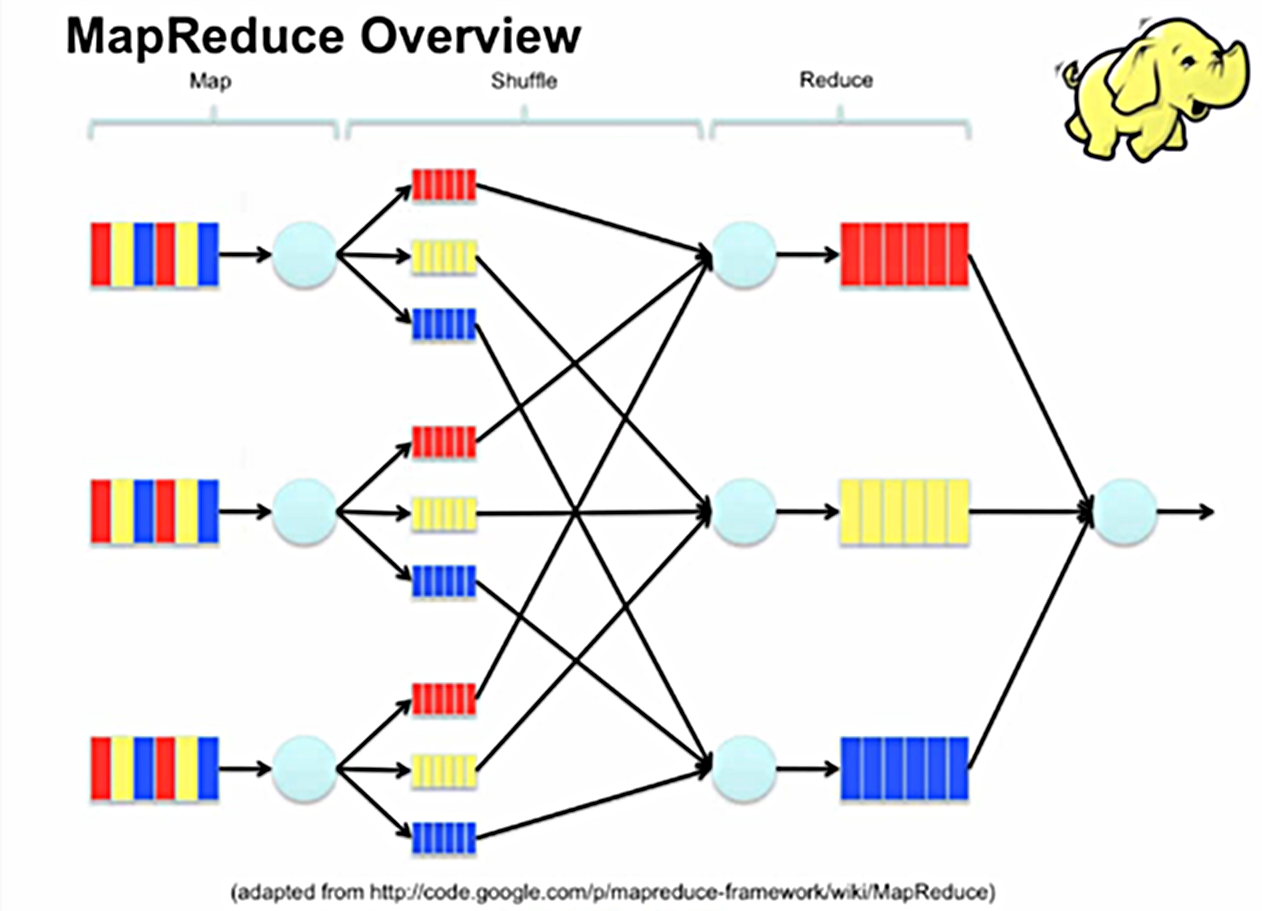
\includegraphics[width=.9\textwidth]{img/mapreduce1}

\framebreak

(de \url{http://www.milanor.net/blog/an-example-of-mapreduce-with-rmr2/})
\centering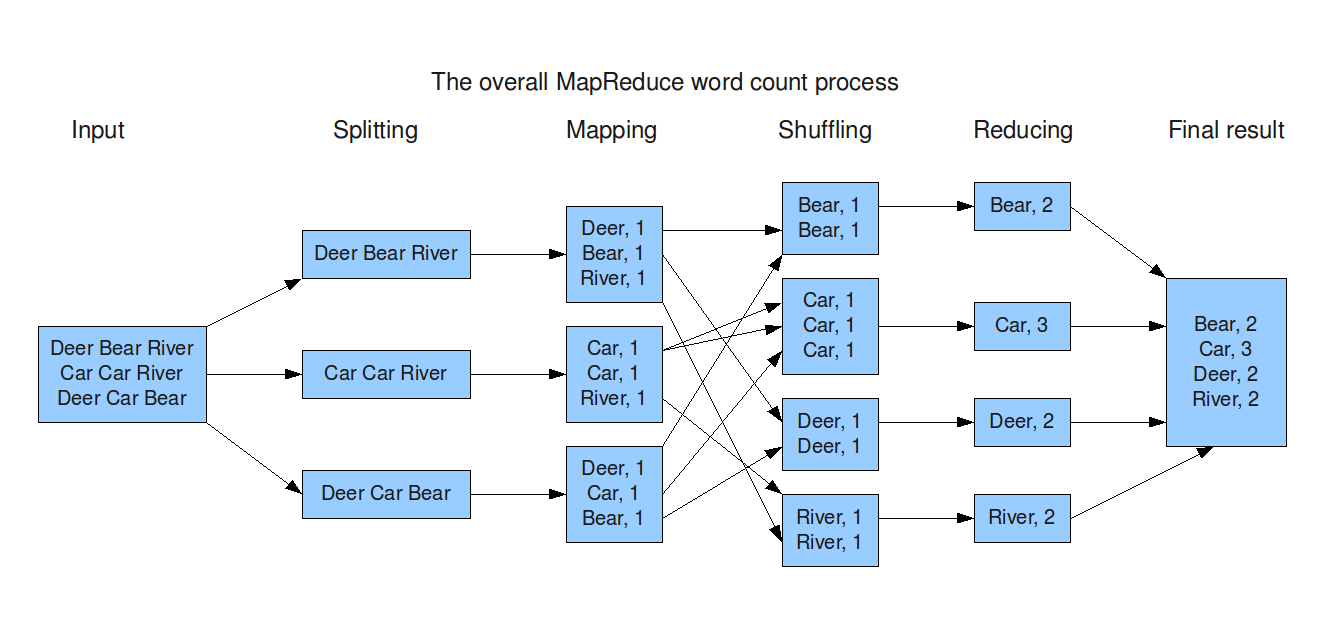
\includegraphics[width=\textwidth]{img/MapReduceWordcount}
\end{frame}

\begin{frame}
\frametitle{Map-Reduce}
\begin{itemize}
\item Map-Reduce en entornos Big-Data/NoSQL
  \begin{itemize}
  \item Entrada \ra{} siempre pares $<key,value>$

  \item {\tt map()} produce otro conjunto de valores
    $\{<key1,value1>,<key2,value2>,...\}$

\item {\em Shuffle} agrupa los valores con la misma clave:
\begin{displaymath}
\{<key1,\{val1,val3,...\}>,<key2,\{val2,val4,...\}>,...\}
\end{displaymath}

\item {\tt reduce()} procesa cada lista de valores con la misma clave, y
  produce otros elementos $<key',value'>$

\item Hay procesamientos difíciles de expresar en Map-Reduce $\Rightarrow$
  varias operaciones M/R {\bf en cadena}
  \end{itemize}
\end{itemize}
\end{frame}


\begin{frame}[fragile,allowframebreaks]
  \frametitle{Map-Reduce y Consultas}
\begin{itemize}
\item Map-Reduce puede usarse no sólo para computación distribuida, sino
  también como una {\bf generalización de consultas}
\item Ejemplo: Imagínese un biólogo marino que hace anotaciones de cada
  animal que ve en el océano, y quiere saber cuántos tiburones ha visto por
  mes:
\begin{lstlisting}[language=SQL]
SELECT MONTH(observation_timestamp) AS observation_month,
       sum(num_animals) AS total_animals
FROM observations
WHERE family = 'Sharks'
GROUP BY observation_month;
\end{lstlisting}

  \framebreak

\item MongoDB con el API de MapReduce:
\begin{lstlisting}[language=Javascript,basicstyle=\footnotesize\tt]
db.observations.mapReduce(
  function map() {
    var year = this.observationTimestamp.getFullYear();
    var month = this.observationTimestamp.getMonth() + 1;
    emit(year + "-" + month, this.numAnimals);
  },
  function reduce(key, values) {
    return Array.sum(values);
  },
  {
    query: { family: "Sharks" },
    out: "monthlySharkReport"
  }
);
\end{lstlisting}

\item  MongoDB ofrece además un API alternativo para funciones de agregación:

\begin{lstlisting}[language=Javascript,basicstyle=\footnotesize\tt]
db.observations.aggregate([
  { $match: { family: "Sharks" } },
  { $group: {
    _id: {
       year: { $year: "$observationTimestamp" },
       month: { $month: "$observationTimestamp" }
    },
    totalAnimals: { $sum: "$numAnimals" }
  }
  }
]);
\end{lstlisting}
\end{itemize}
\end{frame}

\begin{frame}[plain]
  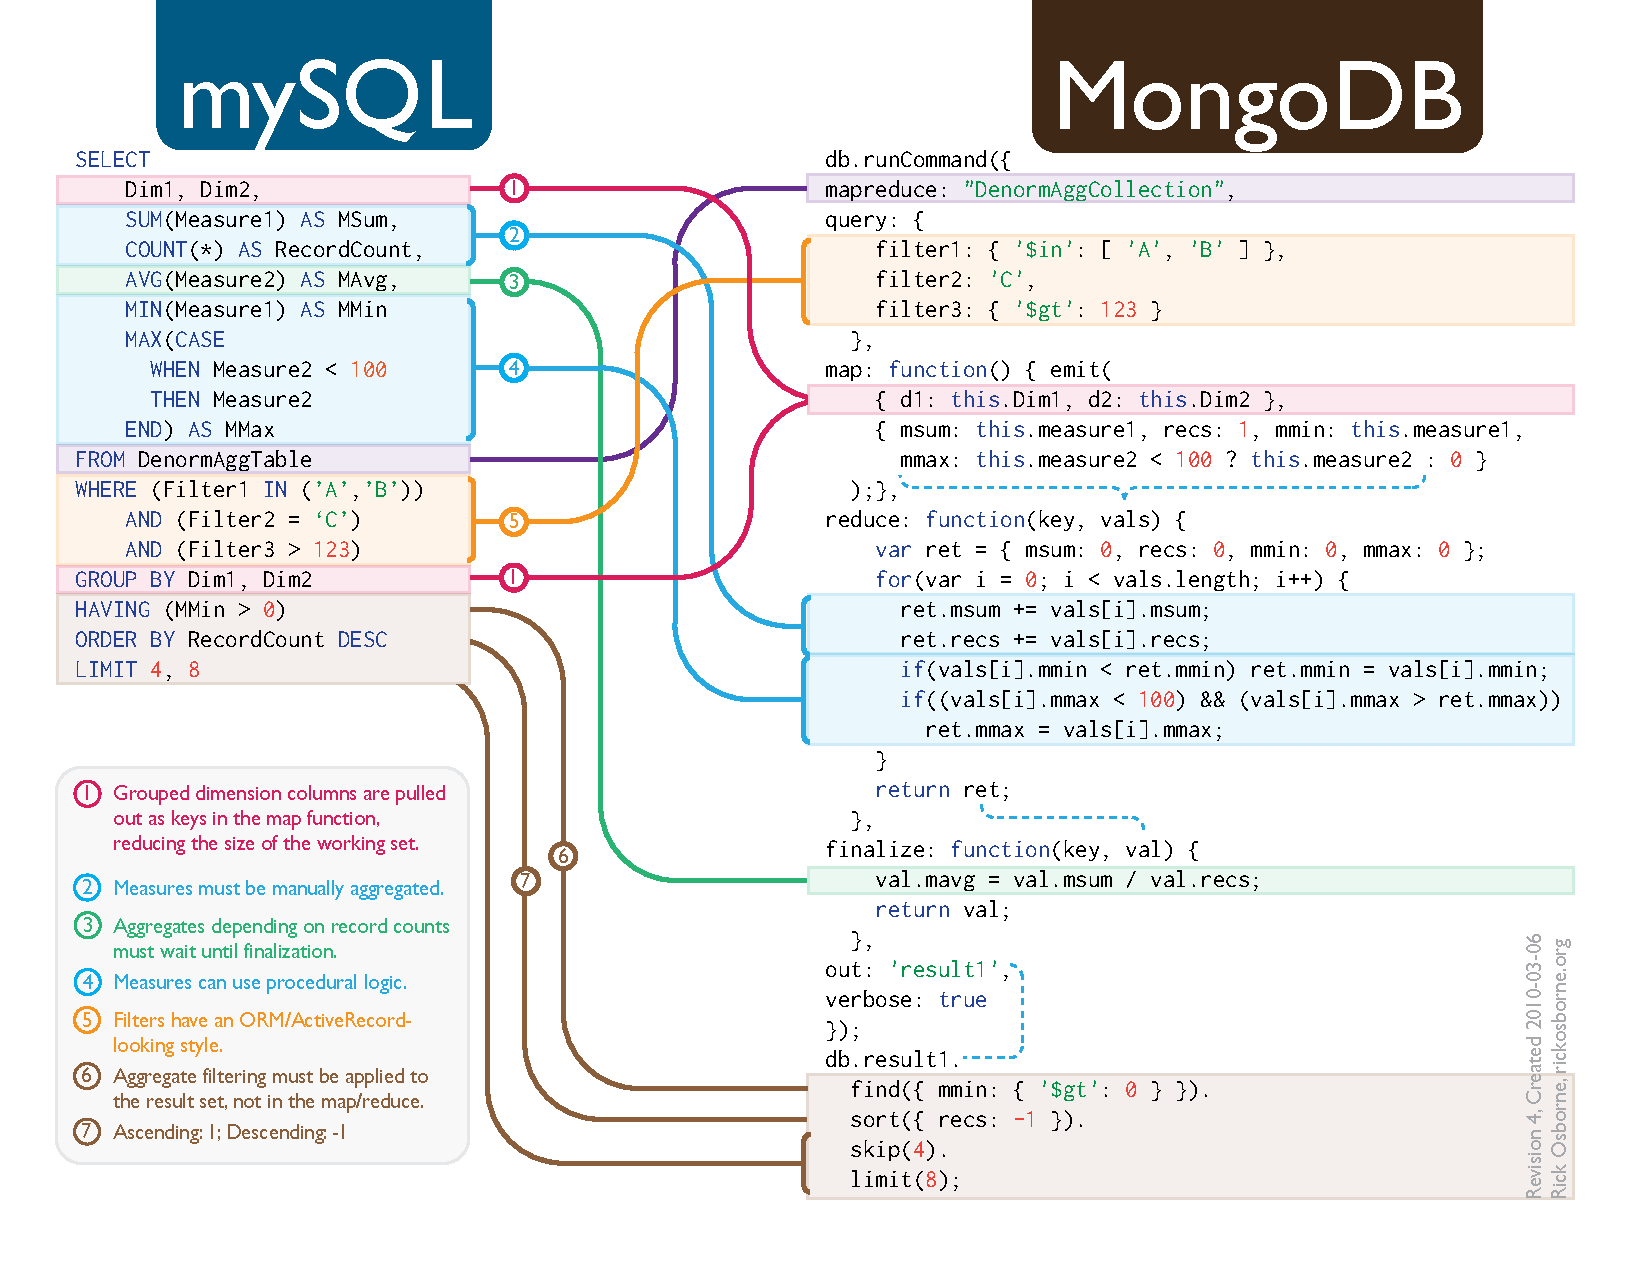
\includegraphics[width=\textwidth]{img/sql-to-mongodb}
\end{frame}

\begin{frame}[fragile,allowframebreaks]
  \frametitle{Uso de MongoDB}
  \begin{itemize}
  \item MongoDB permite el uso desde su {\em shell} o bien desde clientes
    remotos
\begin{verbatim}
$ mongo
MongoDB shell version v3.4.6
connecting to: mongodb://127.0.0.1:27017
MongoDB server version: 3.4.6
>
\end{verbatim}
    \item El shell es básicamente JavaScript, con modificaciones para
      acceder a la base de datos
    \item La variable {\tt db} siempre está disponibles, y guarda la base
      de datos especificada con {\tt use~base-de-datos}
    \item Después, {\tt db.colección} crea la colección ``{\tt colección}''
    \item Dentro de cada colección hay un conjunto de documentos,
      identificados por su campo ``{\tt \_id}''
  \end{itemize}
\end{frame}

\begin{frame}[fragile,allowframebreaks]
  \frametitle{Uso desde {\tt Pymongo}}

\begin{itemize}
\item Para el uso remoto utilizaremos {\tt pymongo}, una biblioteca para
  Python:
\begin{verbatim}
sudo pip2 install pymongo
\end{verbatim}
\item Los nombres de los métodos de las colecciones son muy similares a las
  equivalentes de Javascript
\item Docs:
  \url{http://api.mongodb.com/python/current/api/pymongo/collection.html}
\end{itemize}

\end{frame}

\begin{frame}
  \frametitle{Métodos de búsqueda}
  \begin{itemize}
  \item El método de búsqueda principal es {\tt find()}, que tiene muchas
    opciones
  \item En general permite especificar:

    \begin{itemize}
    \item El filtro de búsqueda
    \item Ordenación de resultados por algún campo
    \item Proyección para no obtener todos los campos del documento
    \item Número de resultados máximo ({\em limit\/})
    \item Número de elementos iniciales a ignorar ({\em skip\/})
    \item El tamaño del {\em batch}
    \end{itemize}

  \item Como la variabilidad es muy grande, veremos ejemplos en la hoja
    Jupyter Notebook y también en la documentación

  \end{itemize}
\end{frame}

\begin{frame}[fragile,allowframebreaks]
  \frametitle{Métodos de búsqueda}
  \begin{itemize}
  \item La función {\tt find()} tiene un gran número de posibilidades para
    especificar la búsqueda. Se pueden utilizar cualificadores complejos
    como:
    \begin{itemize}
    \item \verb|$and|
    \item \verb|$or|
    \item \verb|$not|
    \end{itemize}

  \item Estos calificadores unen ``objetos'', no valores
\framebreak
  \item Por otro lado, hay
    otros calificadores que se refieren a valores:
\begin{itemize}
\item \verb|$lt| (menor)
\item \verb|$lte| (menor o igual)
\item \verb|$gt| (mayor)
\item \verb|$gte| (mayor o igual)
\item \verb|$regex| (expresión regular)
\end{itemize}
  \end{itemize}
\begin{lstlisting}[language=Python]
jisbd17.find_one({'text': {'$regex' : '[Mm]ongo'}})['_id']
\end{lstlisting}
\end{frame}

\begin{frame}
  \frametitle{Métodos de inserción y actualización}
  \begin{itemize}
  \item También ofrece métodos para inserción y actualización:
    \begin{itemize}
    \item {\tt insert\_one()}, {\tt insert\_many()} (batch)
    \item {\tt update\_one()} -- Permite actualizar un objeto con nuevos
      campos. El objeto se crea si se pone el parámetro {\tt upsert} a {\tt
        True}
    \item {\tt update\_many()} -- Permite poner nuevos valores calculados a
      un conjunto de objetos
    \end{itemize}
  \end{itemize}
\end{frame}

\begin{frame}
  \frametitle{Índices, {\tt explain()}}

\end{frame}

\begin{frame}
  \frametitle{Map-Reduce}
  \centering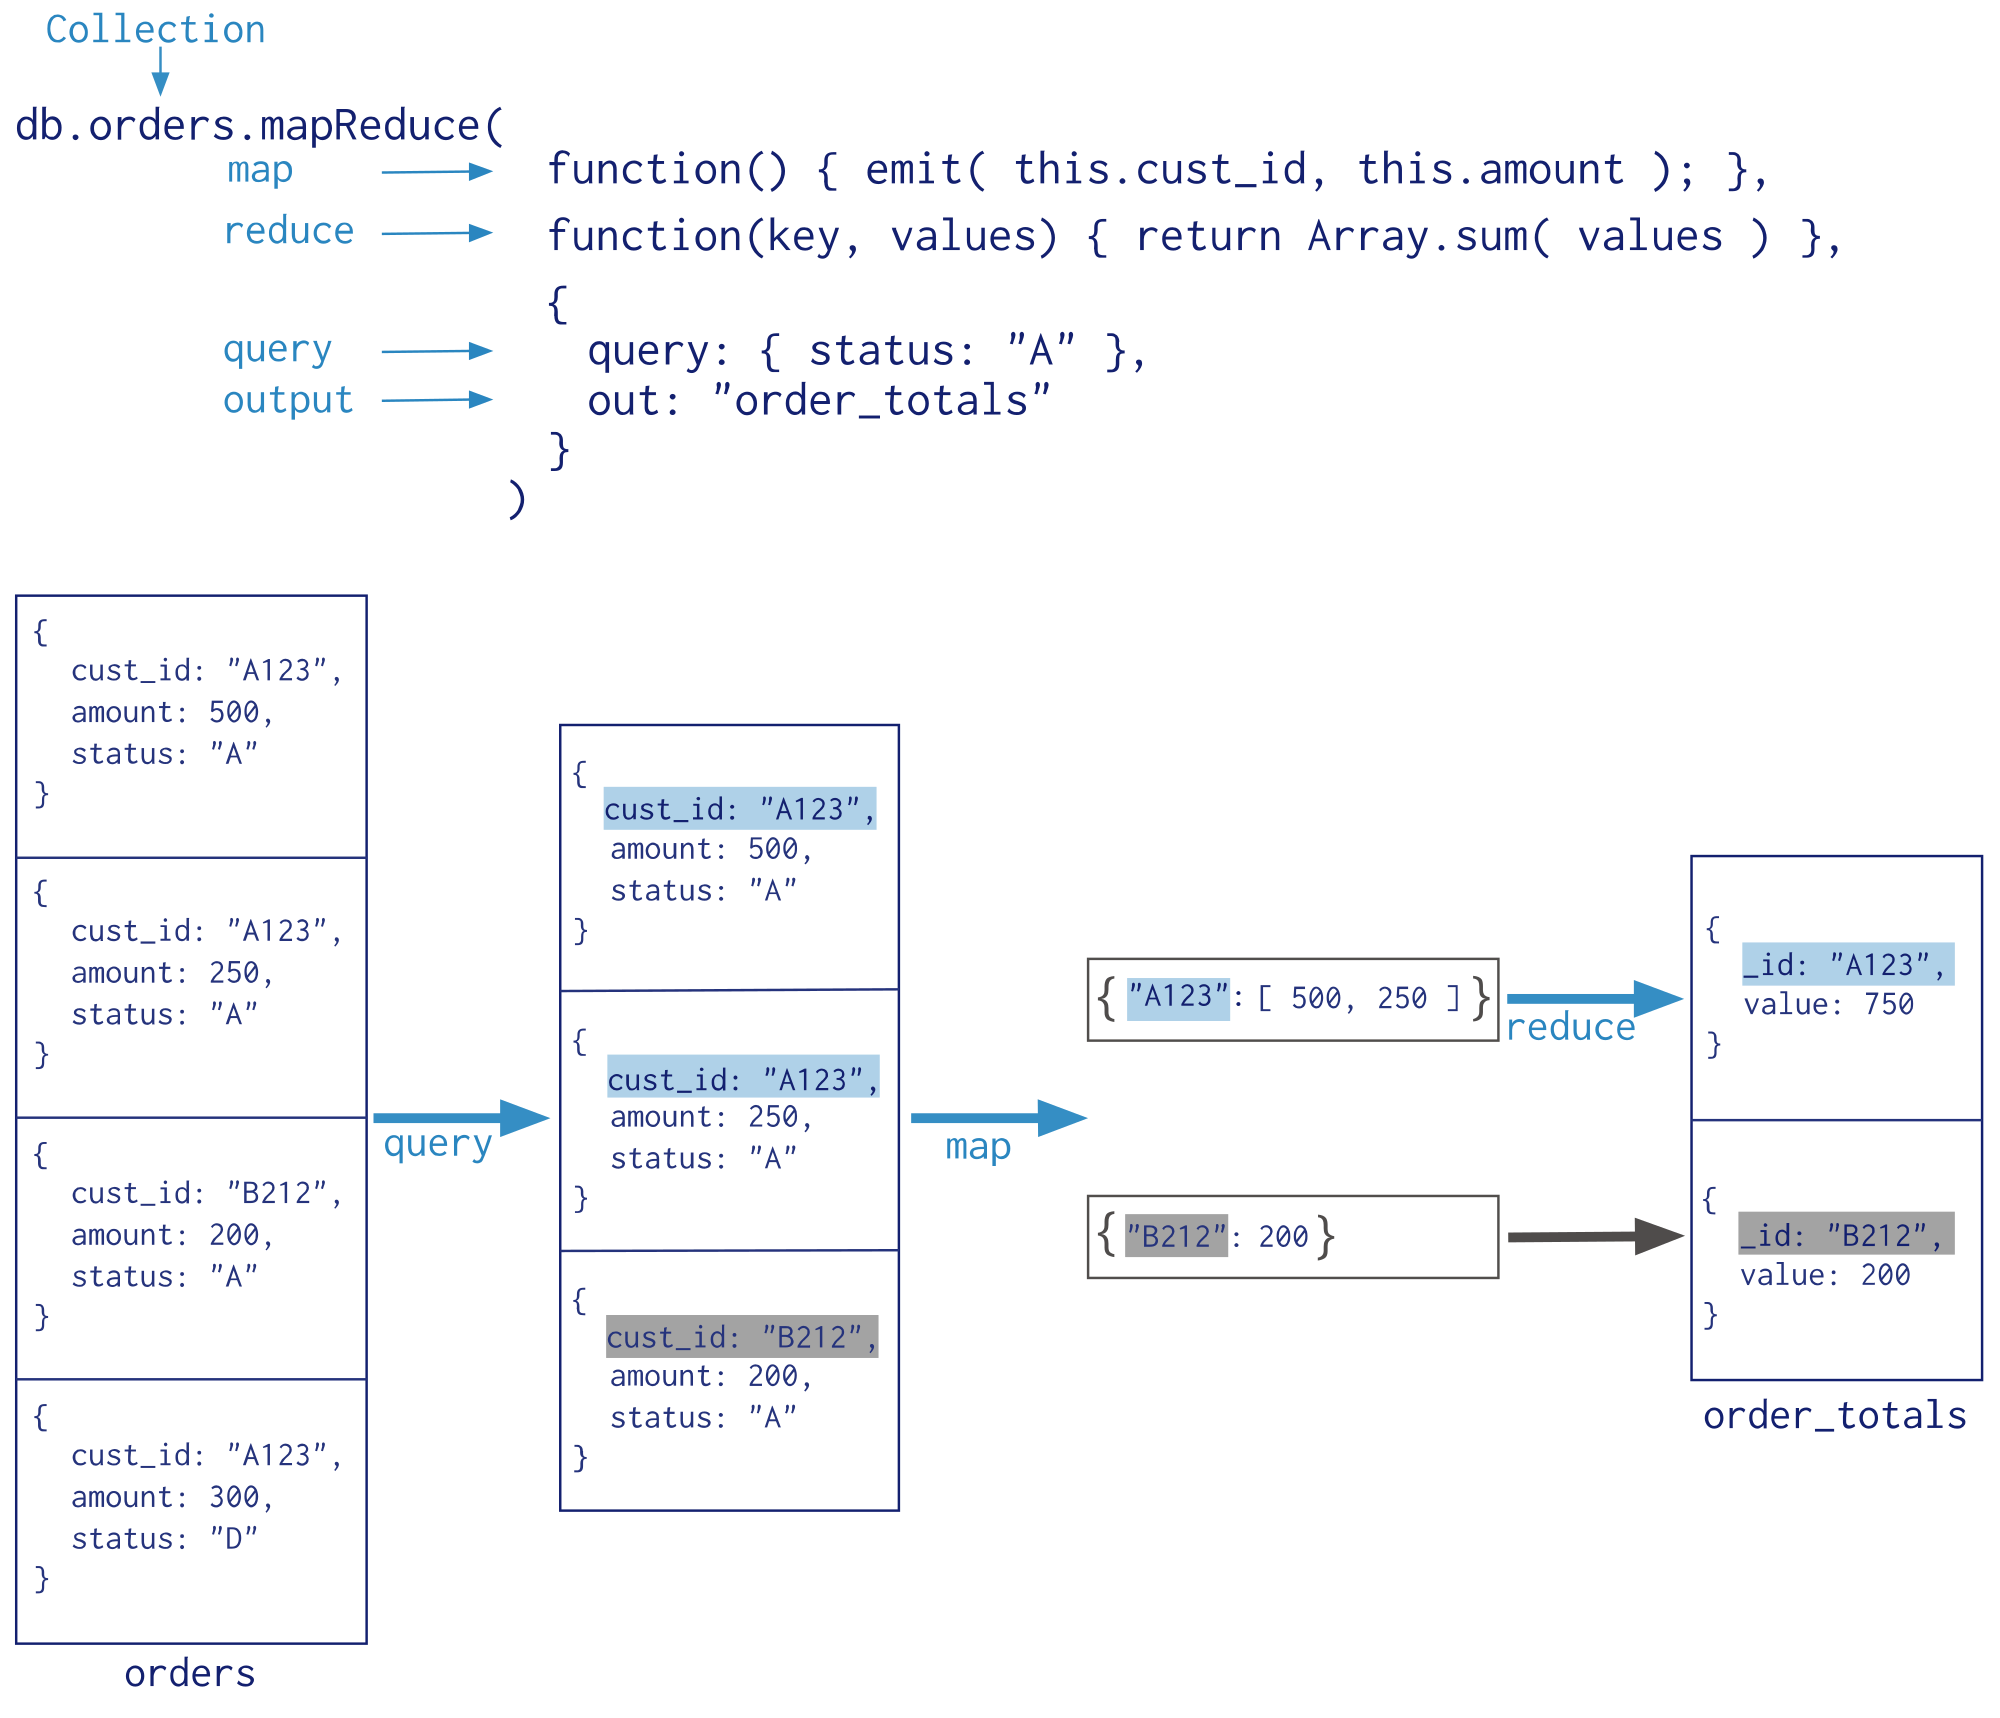
\includegraphics[height=.85\textheight]{img/mongo-map-reduce}
\end{frame}

\begin{frame}
  \frametitle{Framework de agregación}

\end{frame}



\subsection{Bases de Datos Columnares}

\begin{frame}
  \frametitle{Bases de Datos Columnares}
\begin{itemize}
\item Influenciadas por el Paper de Google de 2004 sobre BigTable
\item En general, parecidos a las tablas SQL, salvo que cada fila puede:
  \begin{itemize}
  \item Tener un conjunto de columnas diferente
\item Almacenar {\em series temporales} dentro de una misma fila (varias
  {\em versiones} de un mismo conjunto de columnas)
  \end{itemize}
\item Cada fila tiene un identificador y es un agregado de familias de
  columnas ({\em column family})

\item Cambian el modo de almacenamiento para favorecer ciertas aplicaciones
  (almacenamiento por columnas en vez de por filas)
\item Bases de datos: HBase, Cassandra, Vertica, H-Store
\end{itemize}
\end{frame}

\begin{frame}[plain]
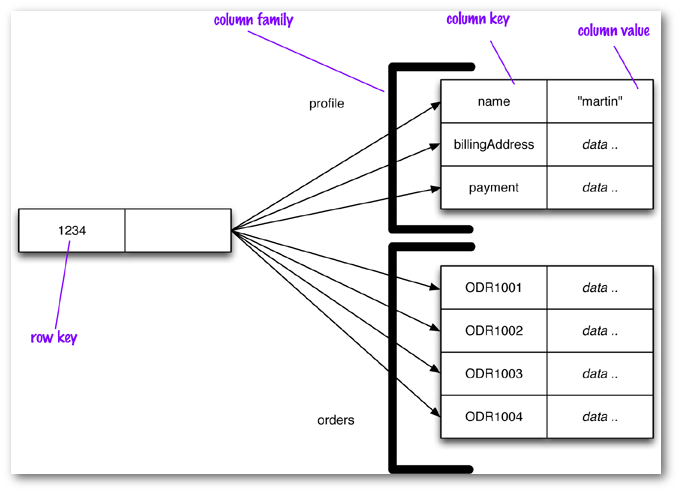
\includegraphics[width=\textwidth]{img/column}
\end{frame}

\begin{frame}[allowframebreaks]
\frametitle{Introducción a HBase}
\begin{center}
  
\includegraphics[width=.5\textwidth]{img/hbase_logo}
\end{center}
\begin{itemize}
\item Base de datos {\em wide column store}
\begin{itemize}
\item Importante: Permite variabilidad en el número de columnas de cada
  fila
\item No sólo crece en número de filas. También puede crecer en número de
  columnas sin coste
\item Es una dimensión más de diseño a tener en cuenta
\item También: Permite almacenar todos los valores antiguos para un dato
  ({\bf series temporales})
\end{itemize}
\item Basada en el artículo seminal de Google sobre ``BigTable'' de
  2006\footnote{Chang, Fay; Dean, Jeffrey; Ghemawat, Sanjay; Hsieh,
    Wilson C; Wallach, Deborah A; Burrows, Michael ‘Mike’; Chandra,
    Tushar; Fikes, Andrew; Gruber, Robert E (2006), {\em Bigtable: A
      Distributed Storage System for Structured Data},
    (\href{http://research.google.com/archive/bigtable-osdi06.pdf}{PDF}),
    Google.}
\item Diseñada para guardar cantidades de datos ingentes en clústers de
  ordenadores
\item Se la nombra como ``La base de datos de Hadoop'', porque sólo depende
  de Hadoop:
  \begin{itemize}
  \item HDFS para almacenar la base de datos de forma distribuida
  \item HDFS permite acceso eficiente para accesos secuenciales y trabajos
    {\em batch\/}
  \item HBase implementa acceso {\em random access} muy rápido
  \item Map/Reduce para realizar búsquedas complejas y procesamiento sobre
    la BD
  \end{itemize}

\framebreak

\item Ofrece casi sólo la funcionalidad de una tabla {\em hash\/} enorme
  con facilidades de tolerancia a fallos y distribución automática y guiada
  \begin{itemize}
  \item Cada fila tiene una clave, por la que se accede
  \item Y un conjunto arbitrariamente grande de columnas, con sus valores
  \item La BD mantiene {\bf físicamente juntas} las claves ordenadas {\bf
      lexicográficamente}
  \item Por lo tanto es {\bf muy rápido} encontrar filas relacionadas
  \item El diseño correcto de la clave es {\color{red} crítico}
  \end{itemize}

\framebreak

\item Operaciones muy rápidas:
  \begin{itemize}
  \item Operaciones CRUD ({\em Create}, {\em Read}, {\em Update}, {\em
      Delete}) rápidas sobre documentos identificados por una clave (se
    implementa alguna versión de árbol B+)
\item Búsqueda secuencial con filtrado, ya que las claves están ordenadas
\item Almacenamiento de un número ilimitado de {\bf versiones de los datos}
  \end{itemize}
  \end{itemize}
\end{frame}

\begin{frame}
  \frametitle{HBase}
  \begin{block}{}
    {\Large  HBase is a {\color{red} sparse},\\ {\color{green} distributed},\\
      {\color{blue} persistent},\\ {\color{red} multi-dimensional} \\
      {\color{green} sorted map} (or Key/Value) \\ {\color{blue} store}}
  \end{block}
\end{frame}

\begin{frame}
  \frametitle{¿Cuándo usar HBase?}

  \begin{block}{}
    Necesidad de realizar cientos, miles de operaciones por segundo en
    TB/PB de datos
  \end{block}

  \begin{block}{}
    Con patrones de accesos son conocidos relativamente bien de antemano y
    no tienen gran complejidad
  \end{block}

\end{frame}

\begin{frame}
  \frametitle{Tecnologías habilitadoras de HBase}
HBase se implementa sobre Hadoop (HDFS y Map-Reduce)
\begin{itemize}
\item Una {\bf tabla} está formada por un número de filas, identificadas
  por una clave
\item Cada tabla se divide en {\bf regiones} (por rangos de clave ordenada
  lexicográficamente) ({\bf partición horizontal})
\item Una instalación de HBase utiliza un conjunto de {\bfseries\itshape
    Region Servers}: nodos de computación con almacenamiento local (y
  conectados al clúster HDFS)
\item Cada grupo de columnas (llamado {\bfseries\itshape Column~Family\/})
  se almacena en un {\bf Store} ({\bf partición vertical})
\item El {\bf Store} tiene una parte en memoria ({\bf MemStore}) y,
  opcionalmente, un almacenamiento en disco, ({\bf HFile})
\item Los {\bf HFile} se distribuyen usando HDFS para lograr replicación y
  tolerancia a fallos
\end{itemize}
\end{frame}

\begin{frame}[allowframebreaks]
  \frametitle{HDFS}
HDFS posee una arquitectura distribuida:
    \begin{itemize}
    \item {\bf NameNode} -- Almacena información sobre qué partes
      ({\bfseries\itshape Chunks}) tiene cada fichero, y dónde están
      almacenadas (y replicadas)
    \item {\bf Secondary Namenode} -- Sustituto del {\bf NameNode} en caso
      de fallo
    \item {\bf DataNode}s -- Almacenan los {\em chunks\/} de cada fichero.
      Cada {\em chunk} puede estar replicado un número de veces,
      dependiendo de la configuración de HDFS
    \item {\bf Zookeeper} -- Se encarga de mantener una consistencia de
      {\em clúster} (saber qué nodos hay conectados y activos) y
      sincronización de datos
    \end{itemize}
  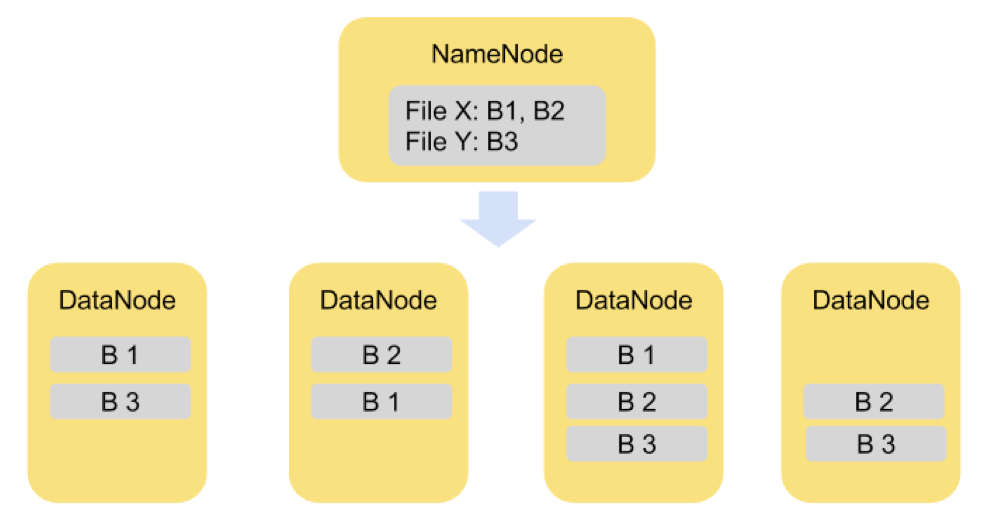
\includegraphics[width=\textwidth]{img/hdfs1}
\end{frame}

\begin{frame}
  \frametitle{Inciso: {\em Consistent Hashing}}
\framesubtitle{\url{http://blog.carlosgaldino.com/consistent-hashing.html}}
  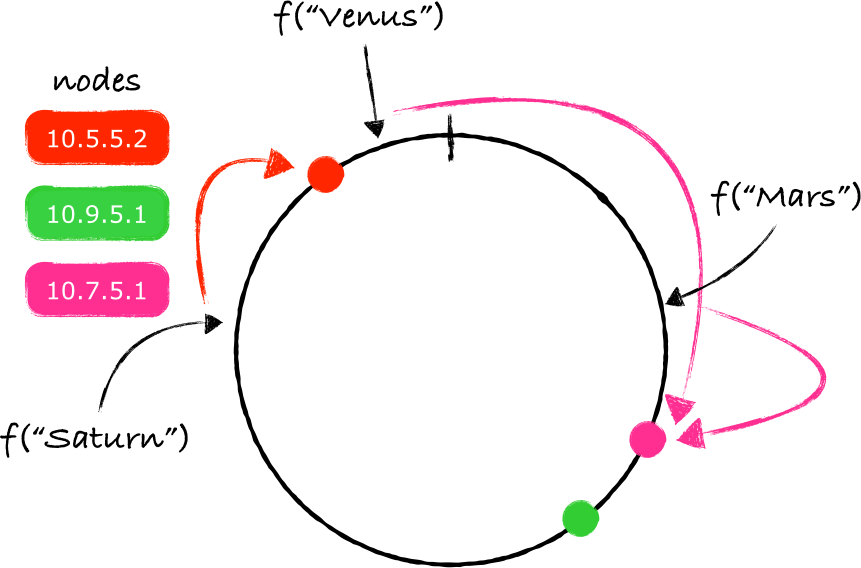
\includegraphics[width=\textwidth]{img/consistent-hashing}
\end{frame}

\begin{frame}
  \frametitle{Inciso: {\em Bloom Filters}}
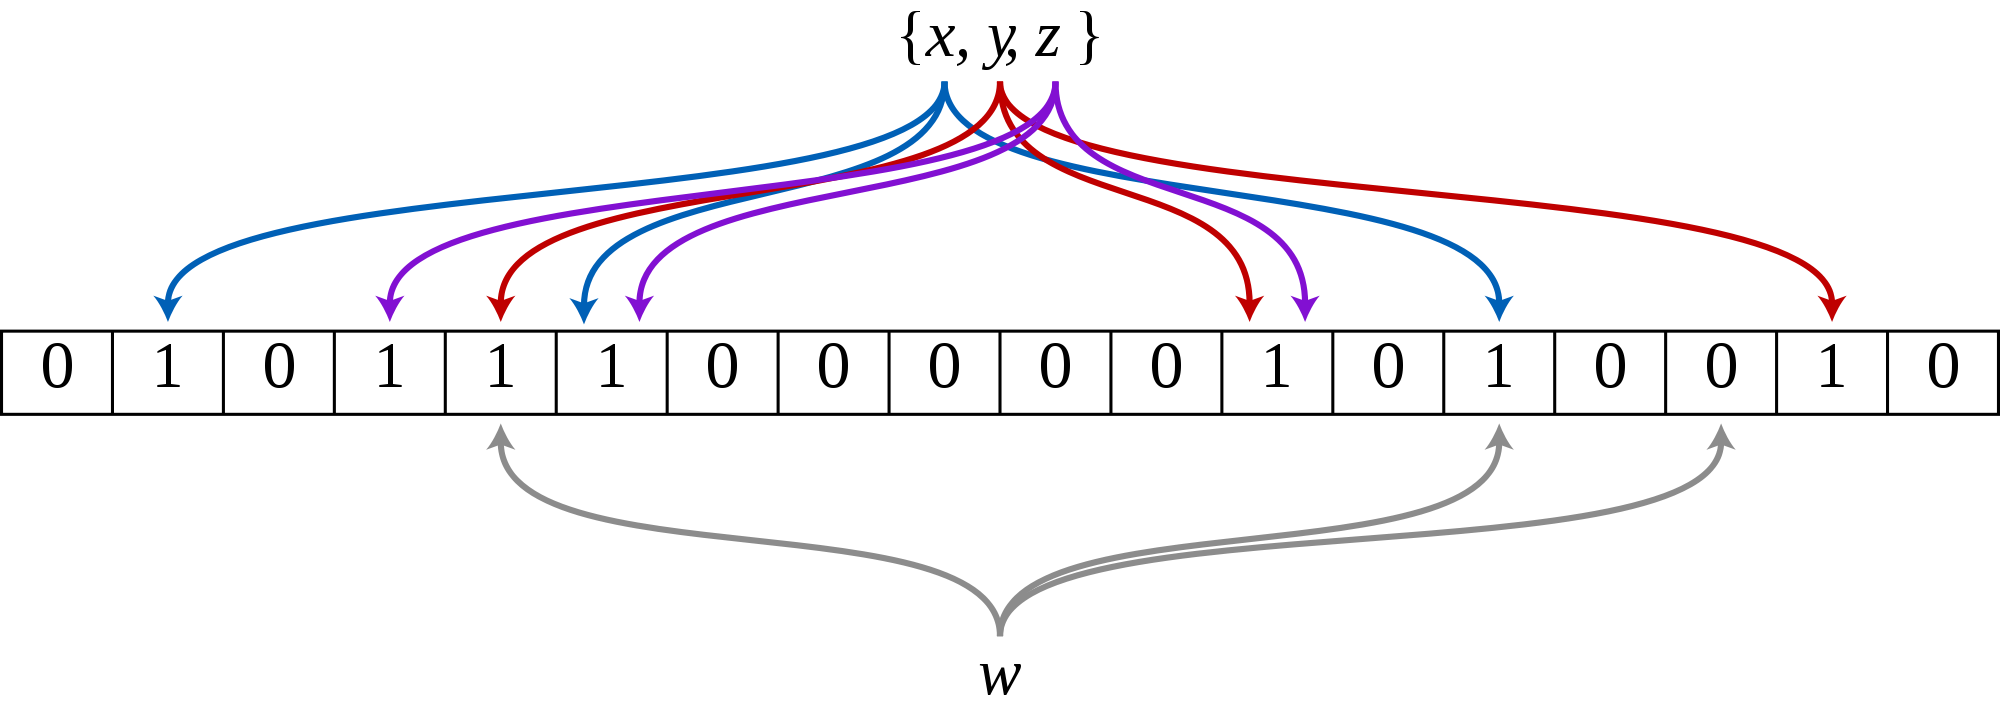
\includegraphics[width=\textwidth]{img/bloom_filter}
\end{frame}

\begin{frame}[allowframebreaks]
  \frametitle{Formato de almacenamiento}
  \begin{itemize}
  \item El formato de HBase es de filas ({\em rows})
\item Cada fila contiene un conjunto especificado de {\em familias de
  columnas}
\item  Cada familia puede incluir un número arbitrario de {\em columnas},
  que puede cambiar por cada fila
\item Para cada valor de columna se pueden guardar opcionalmente varios
  valores anotados con un {\em timestamp} (histórico)
  \end{itemize}
\end{frame}

\begin{frame}[fragile,allowframebreaks]
  \frametitle{Hbase Shell}
\framesubtitle{Comandos básicos CRUD}
\begin{itemize}
\item Versión, estado:

\begin{lstlisting}[language=ruby]
hbase> version
1.1.7, re7ee6fa201c4fb1962f8928df3d519b70b4ff717, Fri Oct  7 18:36:27 PDT 2016
hbase> status
1 servers, 0 dead, 2.0000 average load
\end{lstlisting}

\framebreak

\item Creación de tablas, especificando las {\em column families}
  iniciales:
\begin{lstlisting}[language=ruby]
hbase> create 'publications', 'bibdata', 'abstract', 'text', 'references'
0 row(s) in 1.8480 seconds
=> Hbase::Table - publications
\end{lstlisting}

\item Se crea la tabla {\tt publications} con cuatro familias de columnas,
  {\tt bibdata}, que guardará los datos bibliográficos, {\tt abstract}, que
  guarda el texto del {\em abstract\/}, {\tt text}, que guardará el texto
  del artículo, y {\tt references}, que guarda las citas del artículo

\framebreak

\item Inserción de valores. El {\em shell\/} es limitado y sólo permite
  añadir una columna a la vez:
\begin{lstlisting}[language=ruby,basicstyle=\scriptsize\tt]
hbase> put 'publications', 'My First Paper Title', 'bibdata:year', 2015
0 row(s) in 0.2320 seconds
hbase> put 'publications', 'My First Paper Title', 'bibdata:month', 'June'
0 row(s) in 0.0430 seconds
hbase> put 'publications', 'My First Paper Title', 'abstract:', 'blah blah the abstract'
0 row(s) in 0.0090 seconds
hbase> put 'publications', 'My First Paper Title', 'text:', 'much more blah blah in the text'
0 row(s) in 0.0070 seconds
\end{lstlisting}

  (el formato de especificación es {\bf familia:columna})

\framebreak

\item Obtener el documento:

\begin{lstlisting}[language=ruby,basicstyle=\tiny\tt]
hbase> get 'publications', 'My First Paper Title'
COLUMN                CELL
 abstract:            timestamp=1449240855126, value=blah blah the abstract
 bibdata:month        timestamp=1449240842660, value=June
 bibdata:year         timestamp=1449240826958, value=2015
 text:                timestamp=1449240868170, value=much more blah blah in the
                      text
4 row(s) in 0.5160 seconds
\end{lstlisting}

\framebreak

\item O toda la tabla:
\begin{lstlisting}[language=ruby,basicstyle=\tiny\tt]
hbase> scan 'publications'
ROW                   COLUMN+CELL
 My First Paper Title column=abstract:, timestamp=1449240855126, value=blah blah
                       the abstract
 My First Paper Title column=bibdata:month, timestamp=1449240842660, value=June
 My First Paper Title column=bibdata:year, timestamp=1449240826958, value=2015
 My First Paper Title column=text:, timestamp=1449240868170, value=much more bla
                      h blah in the text
1 row(s) in 0.0450 seconds
\end{lstlisting}
\end{itemize}

\end{frame}

\begin{frame}[allowframebreaks]
  \frametitle{Opciones de tablas}
\begin{itemize}
\item {\tt VERSIONS} es por defecto 1, y se pueden especificar todas o un
  número finito de ellas
\item En el caso de la familia {\tt text}, aplicamos compresión, ya que la
  familia albergará gran cantidad de texto
\item También aplicamos al parámetro {\tt BLOOMFILTER} el valor {\tt ROW}
\framebreak
\item {\tt BLOOMFILTER} puede estar deshabilitado ({\tt NONE}), o tomar dos
  valores:
  \begin{description}[ROW]
  \item[{\tt ROW}] Permite establecer rápidamente si una fila no existe
    \begin{itemize}
    \item Como hemos visto, HBase mantiene una estructura de árbol B+ para
      encontrar las filas buscadas
    \item Sin embargo, el árbol guarda rangos de claves, pero no si una
      clave específica existe o no
    \item Poniendo el valor {\tt ROW}, se crea un filtro Bloom que permite
      descartar cuando una clave no está
    \end{itemize}
\framebreak
  \item[{\tt ROWCOLUMN}] Realiza también un filtro Bloom para describir si
    una columna está en una fila concreta o no. Las columnas pueden ser
    muchas. Además, se utiliza un fichero para cada familia de columnas.
    Por lo tanto, si no se tiene este índice, se tienen que hacer muchas
    comprobaciones para saber si una de las columnas a mostrar está en una
    fila concreta o no. El filtro Bloom con valor {\tt ROWCOLUMN} crea un
    filtro Bloom para las columnas de cada fila
  \end{description}
\end{itemize}
\end{frame}


\begin{frame}[fragile]
  \frametitle{{\tt happybase}}
  \begin{itemize}
\item Hay varios paquetes para acceder a HBase
\item Incluso podríamos haberlo implementado desde JRuby y el {\em shell\/}
  de HBase
\item Pero lo haremos desde Python ya que lo hemos usado en todo el curso,
  usando la librería {\tt
    happybase}\footnote{\url{https://happybase.readthedocs.io/en/latest/}.}
\item Hace uso del protocolo remoto Thrift
\item Instalada en la máquina virtual. Si no, para instalarla:
\begin{lstlisting}[language=bash]
$ pip install happybase
\end{lstlisting}
\item El API es sencillo, ya que HBase ofrece relativamente pocas
  operaciones
\end{itemize}
\end{frame}

\begin{frame}[fragile]
  \frametitle{Creación de la base de datos}
\begin{lstlisting}[language=python]
try:
    self.connection.create_table(
        "wlinks",
        {
            'from': dict(bloom_filter_type='ROW',max_versions=1),
            'to' : dict(bloom_filter_type='ROW',max_versions=1)
        })
except:
    print ("Database wlinks already exists.")
    pass
\end{lstlisting}
\end{frame}

\begin{frame}
  \frametitle{Búsquedas y filtrado}
\begin{itemize}
\item Como se ha visto, el diseño de las tablas HBase tiene que ir
  orientado a la {\bf optimización de las lecturas}
\item Por lo tanto se tiene que desnormalizar todo lo necesario
\item Se tiene que buscar que con un único acceso se obtenga toda la
  información necesaria
\item Sin embargo, esto no es posible siempre:
  \begin{itemize}
  \item Por ejemplo, se tiene que procesar un conjunto de elementos no
    predeterminado
  \item Se quieren calcular resultados agregados semanales, diarios, etc.
  \end{itemize}
\end{itemize}
\end{frame}

\begin{frame}
  \frametitle{Búsquedas y filtrado}
\begin{itemize}
\item HBase ofrece un lenguaje de filtrado que se puede utilizar para que
  el servidor filtre los resultados
\item Se puede usar desde clientes Thrift remotos (como {\tt happybase}) y
  desde el {\em shell}
\item Es el servidor, en cada región en paralelo, el que realiza el
  filtrado
\item Se gana en escalabilidad horizontal si hay muchos {\tt RegionServer}s
\item Aunque ofrece diversos mecanismos de filtrado, no todos son igual de
  eficientes
\item De hecho, el principal problema es que hay mucha diferencia (hasta el
  punto de hacer algunos impracticables) si no se usan bien
\end{itemize}
\end{frame}

\begin{frame}
  \frametitle{Búsquedas y filtrado}
  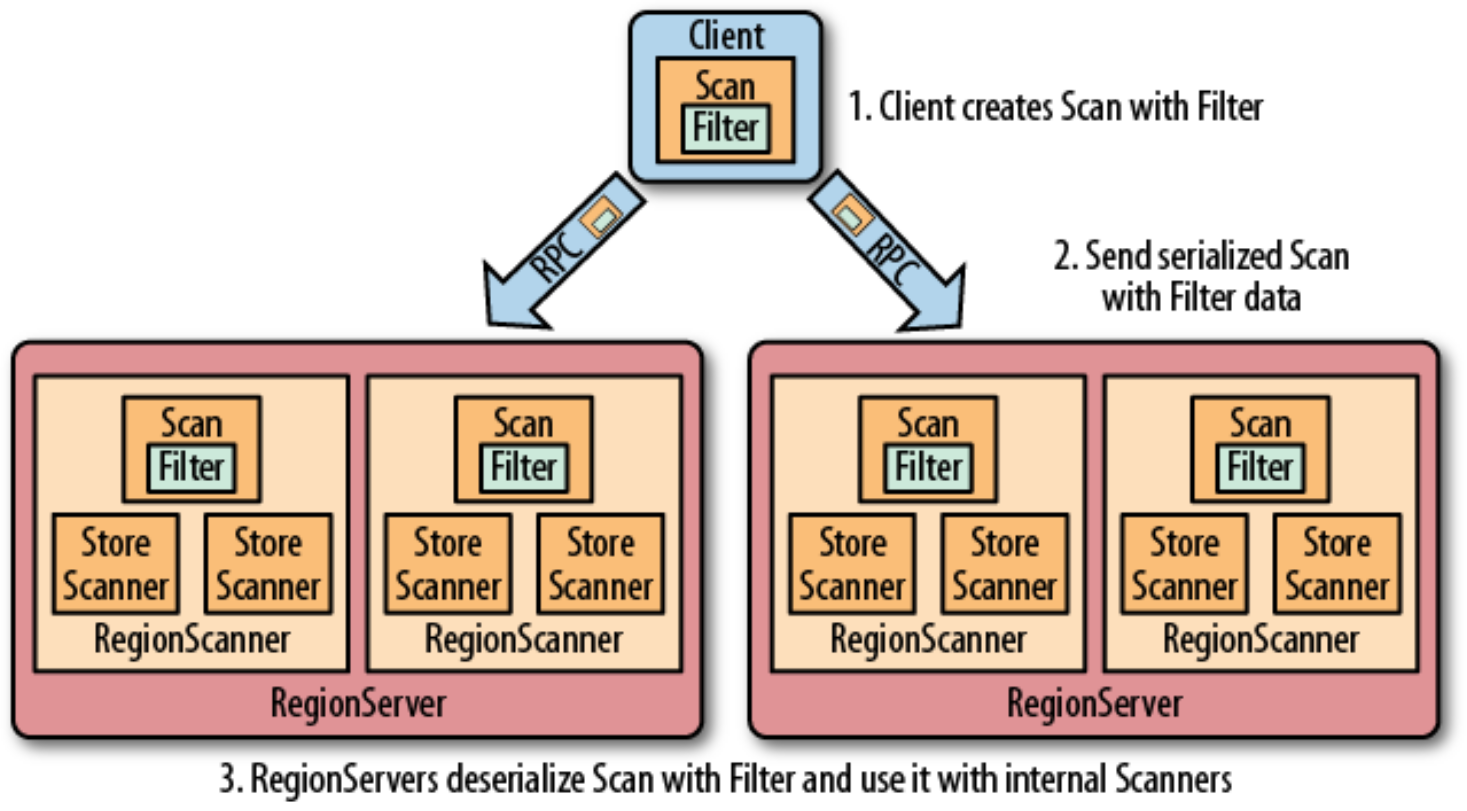
\includegraphics[width=\textwidth]{img/filter-region-server}
\end{frame}

\begin{frame}[fragile]
  \frametitle{Especificación de filtros}
\begin{itemize}
\item Los filtros se especifican como parte de la llamada {\tt scan}
\item Hay dos niveles de filtrado:
  \begin{itemize}
  \item El referido a columnas, que se especifica con el parámetro {\tt
      COLUMNS} en el {\em shell\/} y {\tt columns=} en {\tt happybase}:

\begin{verbatim}
scan 'tabla', { COLUMNS => ['c1', 'c2'] }
\end{verbatim}

  \item Los filtros completos:

\begin{verbatim}
scan 'tabla' , { FILTER => "Filtro" }
\end{verbatim}

(y se pueden combinar ambos)

  \end{itemize}
\item En las bibliotecas cliente como {\tt happybase} con un parámetro de
  la función {\tt scan}:
\begin{lstlisting}
table.scan(filter="Filtro...")
\end{lstlisting}
\end{itemize}
\end{frame}

\begin{frame}[fragile]
  \frametitle{Especificación de filtros (ii)}
\begin{itemize}
\item Así, las consultas se pueden ordenar en cuanto a su velocidad de
  ejecución:
  \begin{enumerate}
  \item Consultas de orden constante, como {\tt get} con un conjunto de
    columnas
  \item Consultas rápidas porque hacen uso de los filtros Bloom: Prefijos
    de claves, familias de columnas, prefijos de familias de columnas, etc
  \item Resto de consultas más lentas, que requieren en algunos casos el
    recorrido de toda la tabla (a evitar): Búsqueda por un valor en
    concreto, búsqueda de expresiones regulares, etc.\\
    (Aunque todavía se benefician del escaneo en paralelo de todas las
    regiones en RegionServers)
  \end{enumerate}
\end{itemize}
\end{frame}


\begin{frame}[fragile,allowframebreaks]
  \frametitle{Sintaxis de filtros}
  \begin{itemize}
  \item La sintaxis general de los filtros es:

\begin{verbatim}
Filtro (parámetro1, parámetro2, ...)
\end{verbatim}

  \item Los filtros se pueden unir con expresiones complejas que incluyan
    paréntesis y también los operadores {\tt AND}, {\tt OR}, {\tt SKIP} y
    {\tt WHILE}
    \begin{itemize}
    \item {\tt SKIP} especifica que se ignore la fila si falla el filtro
      alguno de los pares columna/valor
    \item {\tt WHILE} muestra todos los conjuntos columna/valor de cada
      fila hasta que un conjunto no cumple el filtro
    \end{itemize}

  \item Se ofrecen también operaciones de comparación: \verb|<|, \verb|<=|,
    \verb|=|, \verb|!=|, \verb|>=|, etc.

\framebreak

  \item Y un conjunto de ``comparadores'':

    \begin{itemize}
    \item {\em BinaryComparator} -- Comparador binario lexicográfico de
      elementos. Se representa con ``{\tt binary}''
    \item {\em BinaryPrefixComparator} -- Comaprador binario de prefijos.
      Se representa con ``{\tt binaryprefix}''
    \item {\em RegexStringComparator} -- Comparador de cadenas usando una
      expresión regular: ``{\tt regexstring}''
    \item {\em SubStringComparator} -- Comparador de subcadena: ``{\tt
        substring}''
    \end{itemize}

\framebreak

  \item El formato de especificación es:

\begin{verbatim}
comparador:valor
\end{verbatim}

    Por ejemplo:

    \begin{itemize}
    \item {\tt binary:abc}
    \item {\tt binaryprefix:abc}
    \item {\tt regexstring:ab*c*}
    \item {\tt substring:def}
    \end{itemize}

  \end{itemize}
\end{frame}

\begin{frame}[fragile,allowframebreaks]
  \frametitle{Filtros}

  \begin{itemize}
  \item {\tt KeyOnlyFilter} -- No acepta argumentos y retorna sólo las
    claves de los pares clave/valor:

\lstset{basicstyle=\tiny\tt}

\begin{lstlisting}
hbase> scan 'tags', {FILTER => "KeyOnlyFilter()"}
...
 998                  column=rawdata:Count, timestamp=1479423572196, value=
 998                  column=rawdata:ExcerptPostId, timestamp=1479423572196, val
                      ue=
 998                  column=rawdata:TagName, timestamp=1479423572196, value=
 998                  column=rawdata:WikiPostId, timestamp=1479423572196, value=
\end{lstlisting}

\item {\tt FirstKeyOnlyFilter} -- Retorna sólo la primera clave de cada
  fila

  \framebreak

  \item {\tt PrefixFilter} -- Prefijo de fila dado:

    \begin{lstlisting}
hbase> scan 'tags', {FILTER => "PrefixFilter('9')"}
...
 998                  column=rawdata:TagName, timestamp=1479423572196, value=saf
                      ari
 998                  column=rawdata:WikiPostId, timestamp=1479423572196, value=
                      17125
\end{lstlisting}

  \item {\tt ColumnPrefixFilter} -- Prefijo de columna dado:

\begin{lstlisting}
hbase> scan 'tags', {FILTER => "ColumnPrefixFilter('W')"}
 995                  column=rawdata:WikiPostId, timestamp=1479423572195, value=
 996                  column=rawdata:WikiPostId, timestamp=1479423572195, value=
                      15828
 998                  column=rawdata:WikiPostId, timestamp=1479423572196, value=
                      17125
\end{lstlisting}

    \framebreak

\item {\tt MultipleColumnPrefixFilter} -- (lista)

\item {\tt ColumnCountGetFilter} -- Retorna hasta el número $n$ de columnas
  dado

\item {\tt PageFilter} -- Permite paginación de resultados por clave de
  fila

  \framebreak

\item {\tt RowFilter} -- Coge un operador de comparación y un comparador.
  Si la fila encaja con la comparación, la fila entera si muestra:

\begin{lstlisting}
hbase> scan 'tags', {FILTER => "RowFilter(<,'binary:2')"}
...
 199                  column=rawdata:ExcerptPostId, timestamp=1479423572117, val
                      ue=521
 199                  column=rawdata:TagName, timestamp=1479423572117, value=mav
                      en
 199                  column=rawdata:WikiPostId, timestamp=1479423572117, value=
                      520
\end{lstlisting}

  % MultipleColumnPrefixFilter
% This filter takes a list of column prefixes. It returns key-values that are present in a column that starts with any of the specified column prefixes. Each of the column prefixes must be of the form: “qualifier”.

% ColumnCountGetFilter
% This filter takes one argument – a limit. It returns the first limit number of columns in the table.

% PageFilter
% This filter takes one argument – a page size. It returns page size number of rows from the table.

% ColumnPaginationFilter
% This filter takes two arguments – a limit and offset. It returns limit number of columns after offset number of columns. It does this for all the rows.

% InclusiveStopFilter
% This filter takes one argument – a row key on which to stop scanning. It
% returns all key-values present in rows up to and including the specified
% row.

% TimeStampsFilter
% This filter takes a list of timestamps. It returns those key-values whose timestamps matches any of the specified timestamps.

% RowFilter
% This filter takes a compare operator and a comparator. It compares each row key with the comparator using the compare operator and if the comparison returns true, it returns all the key-values in that row.

\item {\tt FamilyFilter} -- Acepta un operador y un comparador. Muestra
  todas las columnas de familias de las columnas que cumplen el filtro.
  Puede ser rápido si se ha definido un filtro Bloom {\tt ROWCOL} para las
  familias de columnas

\item {\tt QualifierFilter} -- Acepta un operador y un comparador. Muestra
  todas las columnas dentro de cualquier familia de columnas que cumplen el
  filtro. De nuevo, con filtros {\tt ROWCOL} funciona mejor porque puede
  eliminar muchas filas


% Family Filter
% This filter takes a compare operator and a comparator. It compares each column family name with the comparator using the compare operator and if the comparison returns true, it returns all the Cells in that column family.

% QualifierFilter
% This filter takes a compare operator and a comparator. It compares each qualifier name with the comparator using the compare operator and if the comparison returns true, it returns all the key-values in that column.

\item {\tt ValueFilter} -- Acepta un operador y un comparador. Si algún
  valor de algún par clave/valor coincide, se muestran todos los elementos
  de la fila

% ValueFilter
% This filter takes a compare operator and a comparator. It compares each value with the comparator using the compare operator and if the comparison returns true, it returns that key-value.

% DependentColumnFilter
% This filter takes two arguments – a family and a qualifier. It tries to locate this column in each row and returns all key-values in that row that have the same timestamp. If the row doesn’t contain the specified column – none of the key-values in that row will be returned.
  \framebreak

\item {\tt SingleColumnValueFilter} -- Acepta una familia de columnas, un
  calificador de columna, un operador de comparación y un comparador. Si la
  columna no está o está y tiene el valor especificado, se lista toda la
  fila

\begin{lstlisting}
hbase> scan 'tags', {FILTER => "SingleColumnValueFilter('rawdata', 'TagName', =,'binary:safari')"}
ROW                   COLUMN+CELL
 998                  column=rawdata:Count, timestamp=1479423572196, value=2
 998                  column=rawdata:ExcerptPostId, timestamp=1479423572196, val
                      ue=17126
 998                  column=rawdata:TagName, timestamp=1479423572196, value=saf
                      ari
 998                  column=rawdata:WikiPostId, timestamp=1479423572196, value=
                      17125
1 row(s) in 0.0650 seconds
\end{lstlisting}

% SingleColumnValueFilter
% This filter takes a column family, a qualifier, a compare operator and a comparator. If the specified column is not found – all the columns of that row will be emitted. If the column is found and the comparison with the comparator returns true, all the columns of the row will be emitted. If the condition fails, the row will not be emitted.

% SingleColumnValueExcludeFilter
% This filter takes the same arguments and behaves same as SingleColumnValueFilter – however, if the column is found and the condition passes, all the columns of the row will be emitted except for the tested column value.

\item {\tt ColumnRangeFilter} -- Acepta dos valores de columna y dos
  booleanos. Muestra las columnas que están entre los valores. Los
  booleanos especifican si se incluyen los valores límite o no.

% ColumnRangeFilter
% This filter is used for selecting only those keys with columns that are between minColumn and maxColumn. It also takes two boolean variables to indicate whether to include the minColumn and maxColumn or not.

\end{itemize}
\end{frame}

\begin{frame}
  \frametitle{Resumen de filtros y características}
  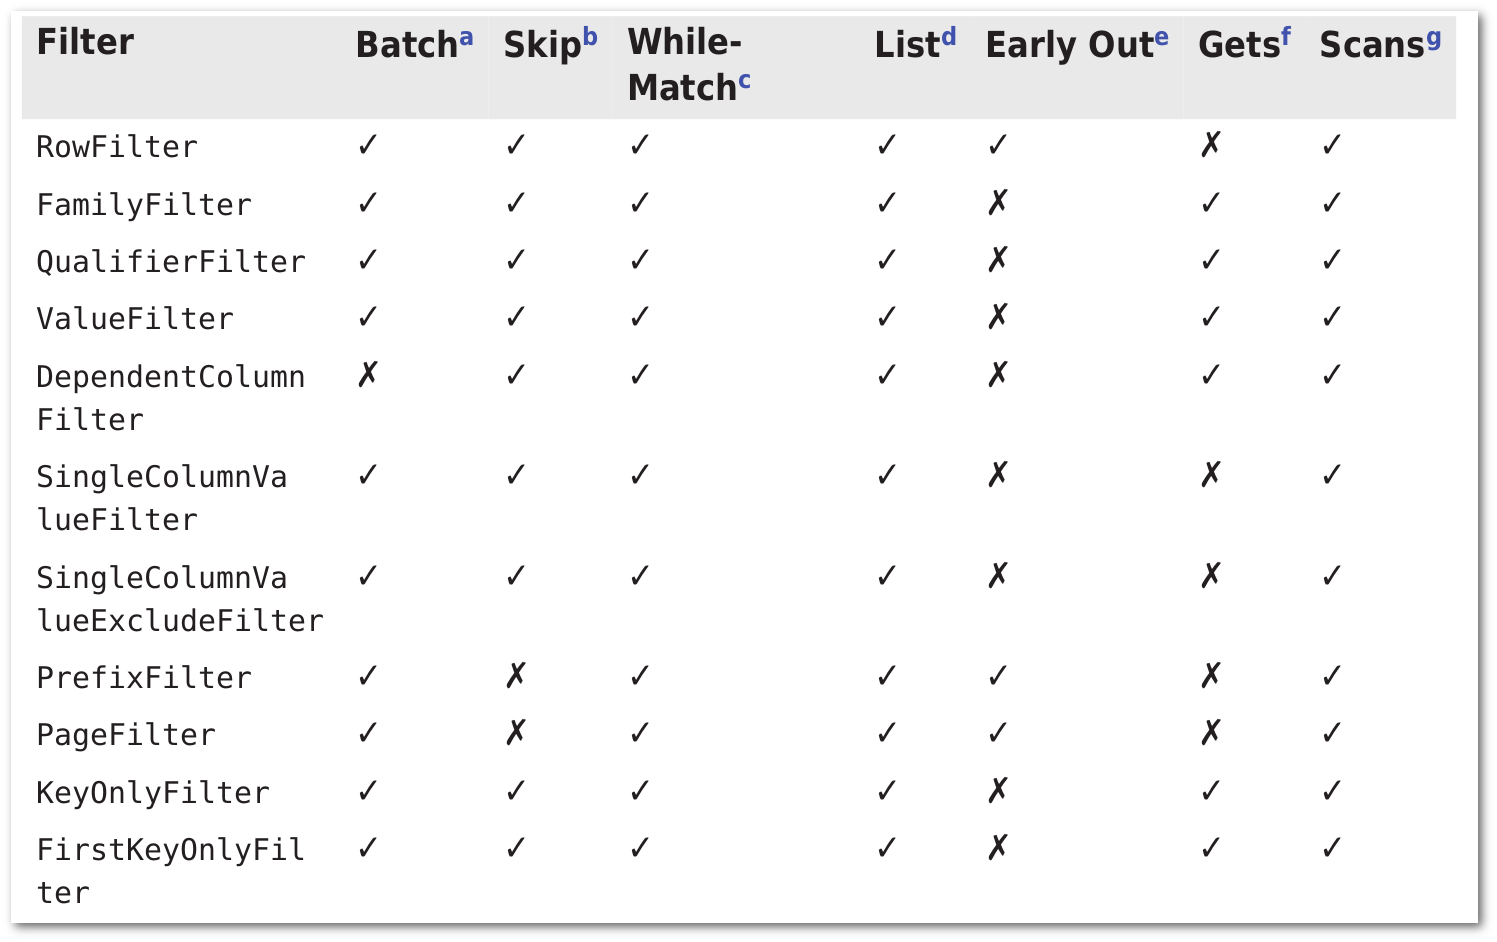
\includegraphics[width=\textwidth]{img/filterlist1}
\end{frame}
\begin{frame}
  \frametitle{Resumen de filtros y características}
  \begin{center}
    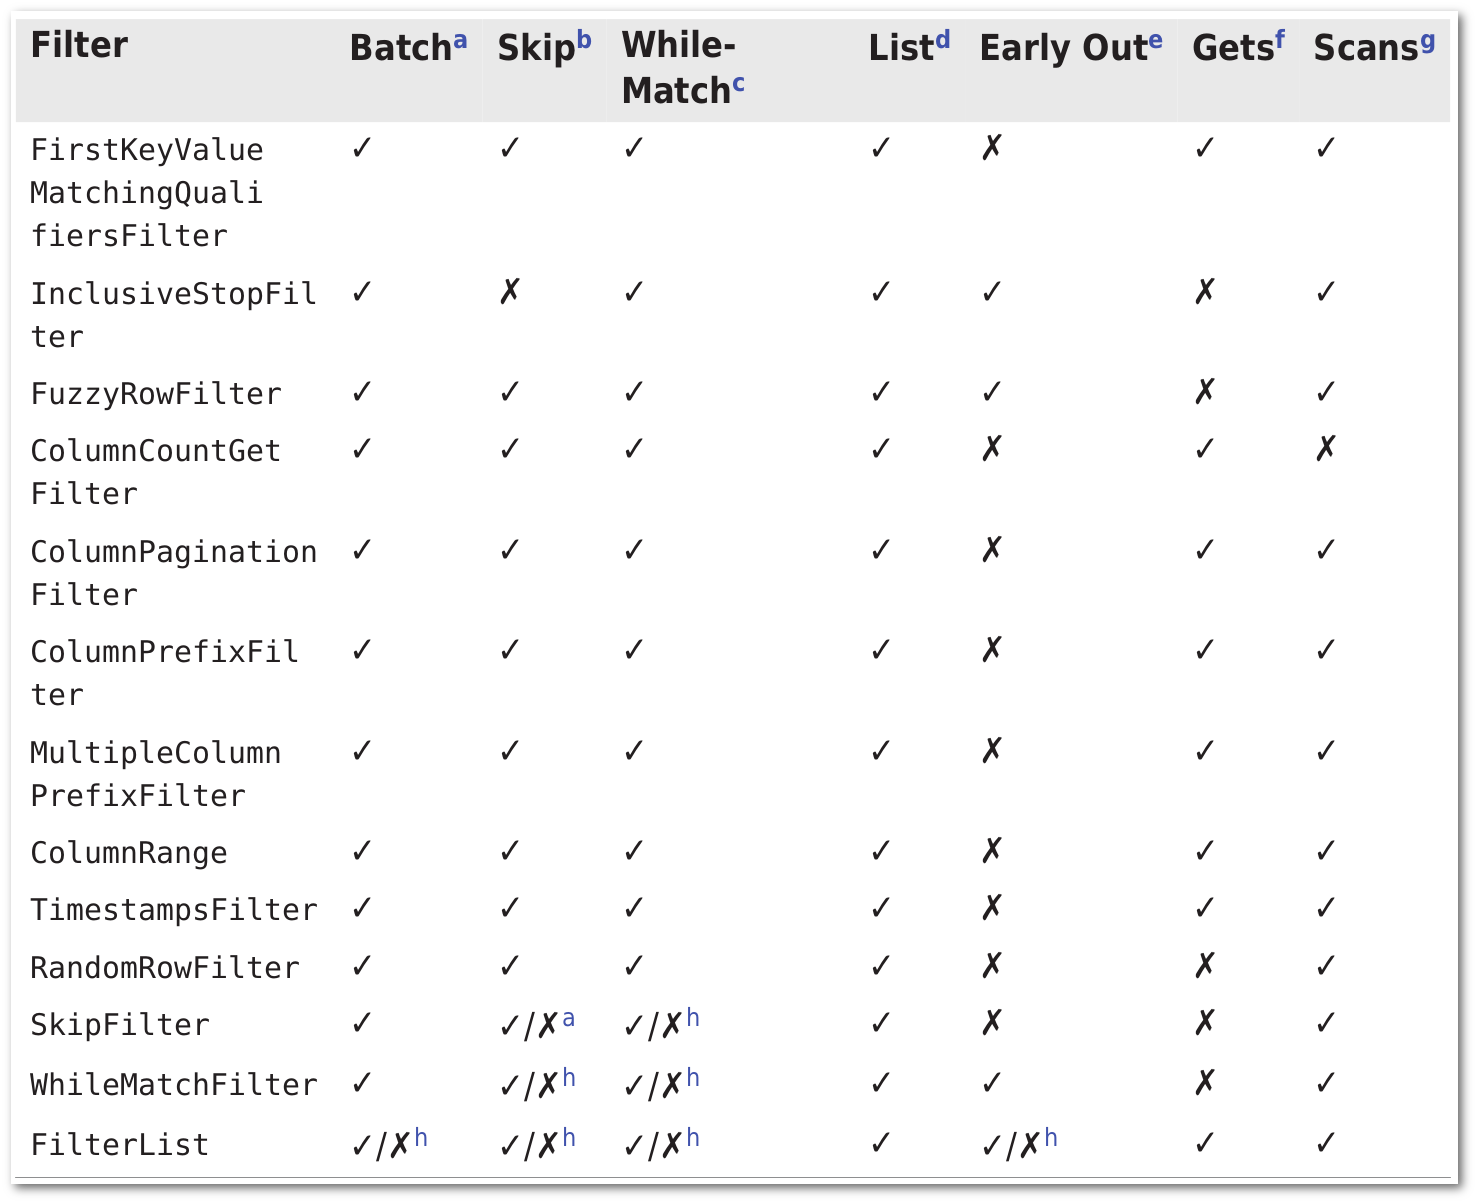
\includegraphics[width=.8\textwidth]{img/filterlist2}
  \end{center}
\end{frame}
\begin{frame}
  \frametitle{Resumen de filtros y características}
  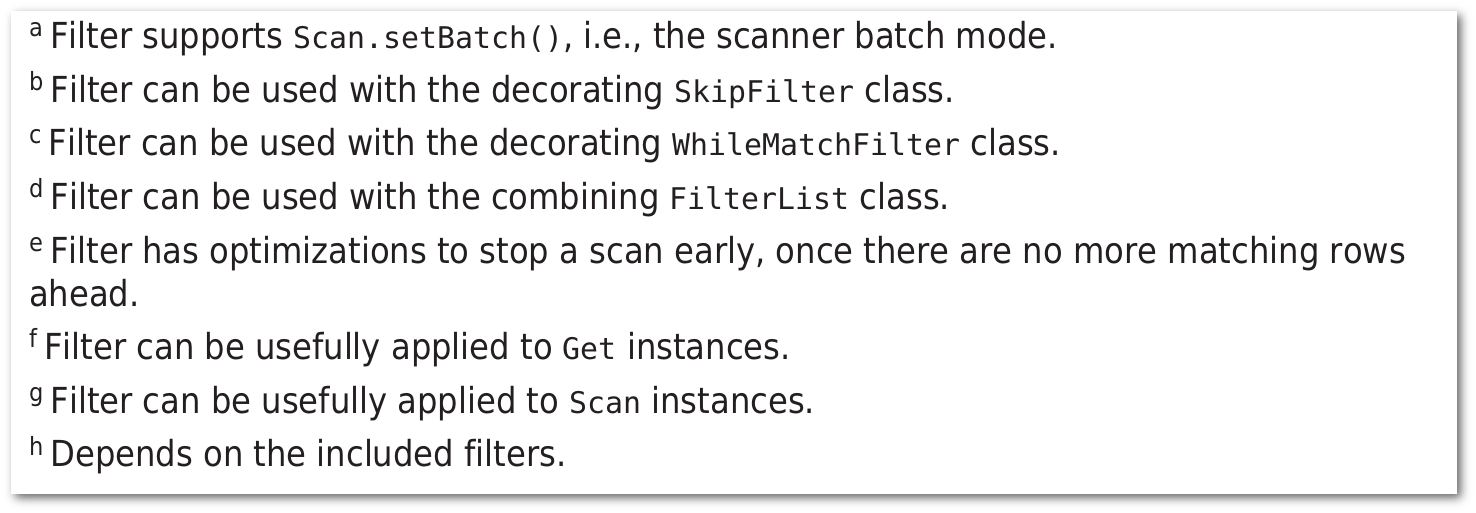
\includegraphics[width=\textwidth]{img/filterlist3}
\end{frame}

\begin{frame}[fragile,allowframebreaks]
  \frametitle{Filtros vs. {\tt get}}
  \begin{itemize}
  \item Por muy eficiente que se haga el filtrado, un {\tt scan} siempre va
    a ser mucho más lento que obtener una fila con {\tt get}
  \item P.ej (3580ms):
\begin{lstlisting}
hbase> scan 'wlinks', { COLUMNS => ['to:19'] }
...
 Yilmar Mosquera      column=to:19, timestamp=1479230326585, value=
 Yukiko Iwai          column=to:19, timestamp=1479230347810, value=
113 row(s) in 35.7690 seconds
\end{lstlisting}

    \framebreak

  \item vs (18ms):
\begin{lstlisting}
hbase> get 'wlinks', '19', { COLUMNS => ['from'] }
...
 from:Yilmar Mosquera timestamp=1479230326578, value=
 from:Yukiko Iwai     timestamp=1479230347796, value=
113 row(s) in 0.1760 seconds
\end{lstlisting}

  \item También existe una especificación de fila de inicio y final que son
    más eficientes que un filtro {\em Row Prefix}:

\begin{lstlisting}
hbase> scan 'wlinks', {STARTROW => '19', ENDROW => '20', COLUMNS => ['from'] }
\end{lstlisting}

    Y en {\tt happybase}:

\begin{lstlisting}[language=Python]
table.scan(row_start='19', row_stop='20', columns=['from'])
\end{lstlisting}

  \end{itemize}
\end{frame}



\subsection{Bases de Datos de Grafos}

\begin{frame}
  \frametitle{Bases de Datos de Grafos}
\vspace*{-1ex}
  \begin{itemize}
  \item Las bases de datos de grafos llevan el mecanismo {\em muchos a
      muchos} al extremo
\item Datos en los que existen muchas relaciones entre sí y
  tienen un significado primordial
\item Las bases de datos de grafos se basan en la construcción y consulta
  de un grafo que consta de
  \begin{itemize}
  \item {\bf Vértices}, también llamados {\em nodos} o {\em entidades}, y
  \item {\bf Aristas} ({\bfseries\itshape Edges}), también llamados {\em
      relaciones}
  \end{itemize}
\item Los grafos pueden capturar relaciones complejas entre
  entidades y ofrecen lenguajes de búsqueda, actualización y creación que
  permiten trabajar con subconjuntos del grafo
% \item Orígenes en las bases de datos de hechos (con lenguajes de consulta
%   lógicos (p. ej. {\em Datalog})
\item Origen en las bases de datos de hechos ({\em Datalog\/})
\item Ejemplos: FlockDB, Neo4J, OrientDB
\end{itemize}
\end{frame}

\begin{frame}[plain]
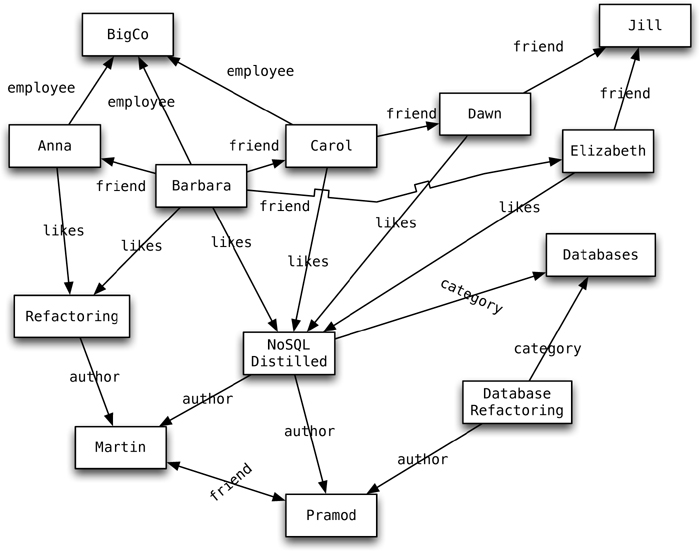
\includegraphics[width=\textwidth]{img/graph}
\end{frame}

\begin{frame}[fragile,plain]
(Nota: Usa la sintaxis PostgreSQL para {\tt json})
\begin{lstlisting}[language=SQL]
CREATE TABLE vertices (
  vertex_id integer PRIMARY KEY,
  properties json
);

CREATE TABLE edges (
  edge_id integer PRIMARY KEY,
  tail_vertex integer REFERENCES vertices (vertex_id),
  head_vertex integer REFERENCES vertices (vertex_id),
  label text,
  properties json
);

CREATE INDEX edges_tails ON edges (tail_vertex);
CREATE INDEX edges_heads ON edges (head_vertex);
\end{lstlisting}
\end{frame}

\begin{frame}[fragile,allowframebreaks]
  \frametitle{Ejemplo de datos y consulta en Neo4J}
\begin{block}{}
\begin{lstlisting}
CREATE
  (NAmerica:Location {name:'North America', type:'continent'}),
  (USA:Location {name:'United States', type:'country' }),
  (Idaho:Location {name:'Idaho', type:'state' }),
  (Lucy:Person {name:'Lucy' }),
  (Idaho)-[:WITHIN]->(USA)-[:WITHIN]-> (NAmerica),
  (Lucy) -[:BORN_IN]-> (Idaho)
\end{lstlisting}
\end{block}

\framebreak

Y de consulta:
\begin{block}{}
\begin{lstlisting}
MATCH
(person) -[:BORN_IN]-> () -[:WITHIN*0..]-> (us:Location {name:'United States'}),
(person) -[:LIVES_IN]-> () -[:WITHIN*0..]-> (eu:Location {name:'Europe'})
RETURN person.name
\end{lstlisting}
\end{block}
\end{frame}


\begin{frame}[allowframebreaks]
  \frametitle{Aplicabilidad de Grafos}
  \begin{itemize}
  \item Los grafos, conceptualmente, aparecen en casi cualquier dominio
  \item Además, su flexibilidad hace que se puedan aplicar de diferentes
    formas
  \item Por ejemplo, una relación de {\em follow\/} entre usuarios:

    \begin{center}
      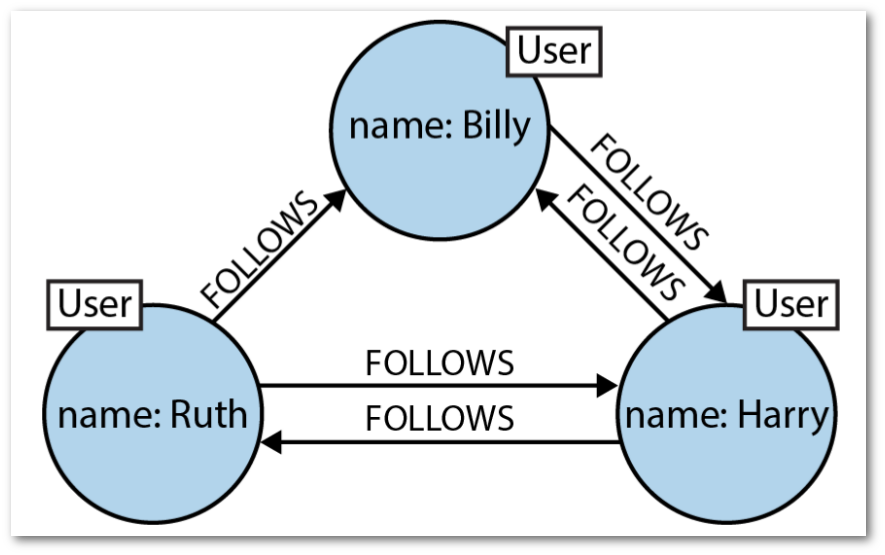
\includegraphics[width=.4\textwidth]{img/graph1}
    \end{center}
  \end{itemize}

    \begin{columns}
      \begin{column}{.5\textwidth}
        \begin{itemize}
      \item (nótese cómo {\bf Billy no ha seguido a Ruth}: las relaciones
        pueden ser unidireccionales o bidireccionales)

      \item Pero también se puede usar para guardar el conjunto de mensajes
        que se intercambian:
      \end{itemize}
    \end{column}
      \begin{column}{.5\textwidth}
        \begin{center}
          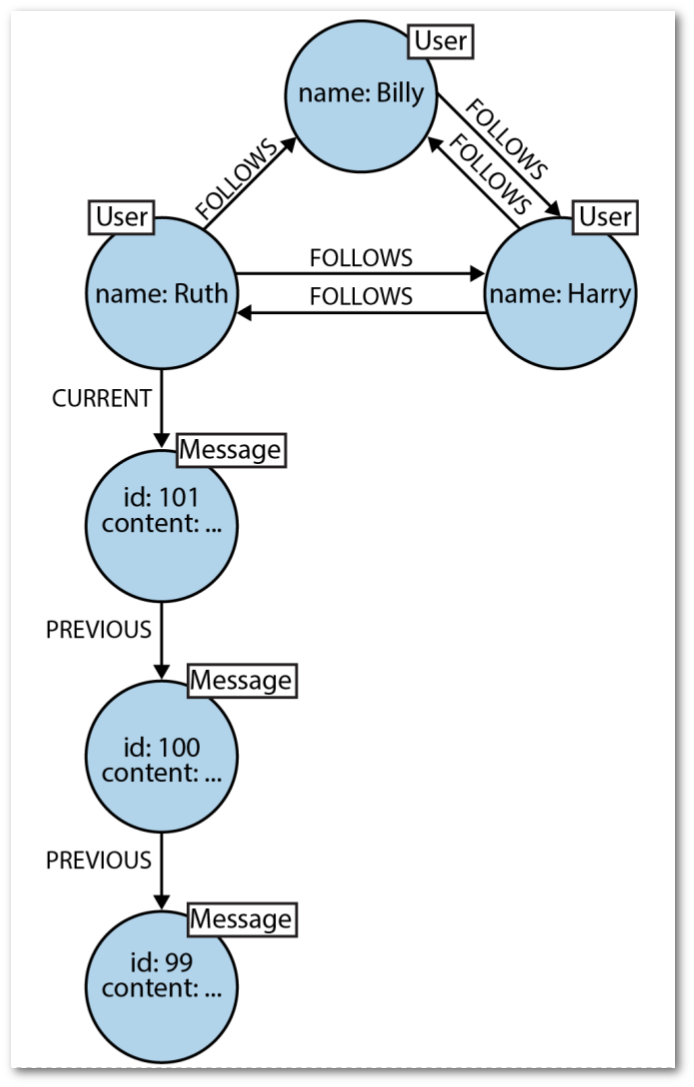
\includegraphics[width=.8\textwidth]{img/graph2}
        \end{center}
      \end{column}
    \end{columns}

  \begin{center}
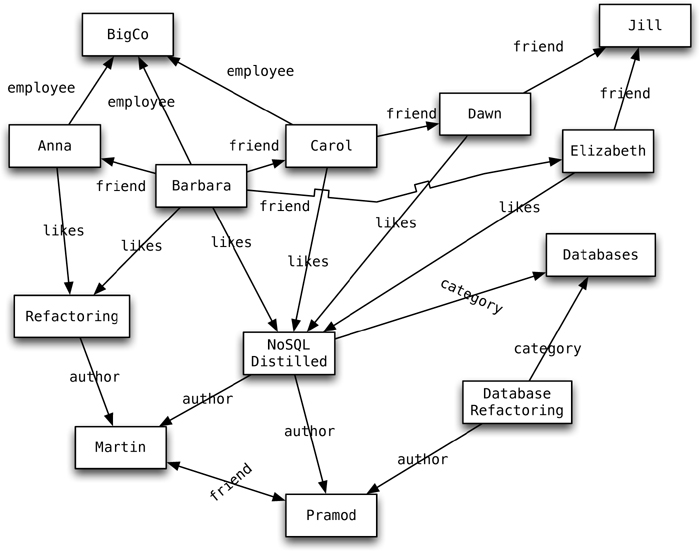
\includegraphics[width=.86\textwidth]{img/graph}
  \end{center}
\end{frame}

\begin{frame}[fragile,allowframebreaks]
  \frametitle{Flexibilidad y eficiencia}
\begin{itemize}
\item Las bases de datos basadas en grafos vienen a suplir dos carencias
  fundamentales:
  \begin{enumerate}
  \item La carencia expresiva del resto de paradigmas para expresar ciertos
    algoritmos que se expresan de forma natural en forma de grafos
  \item La eficiencia del tratamiento de estos procesos en grafos vs. otros
    paradigmas
  \end{enumerate}
\item Como ejemplo, usemos una relación de amistad ({\em friend\/}) entre
  usuarios de una red social
\framebreak
\item Una posible implementación relacional podría ser:
  \begin{center}
    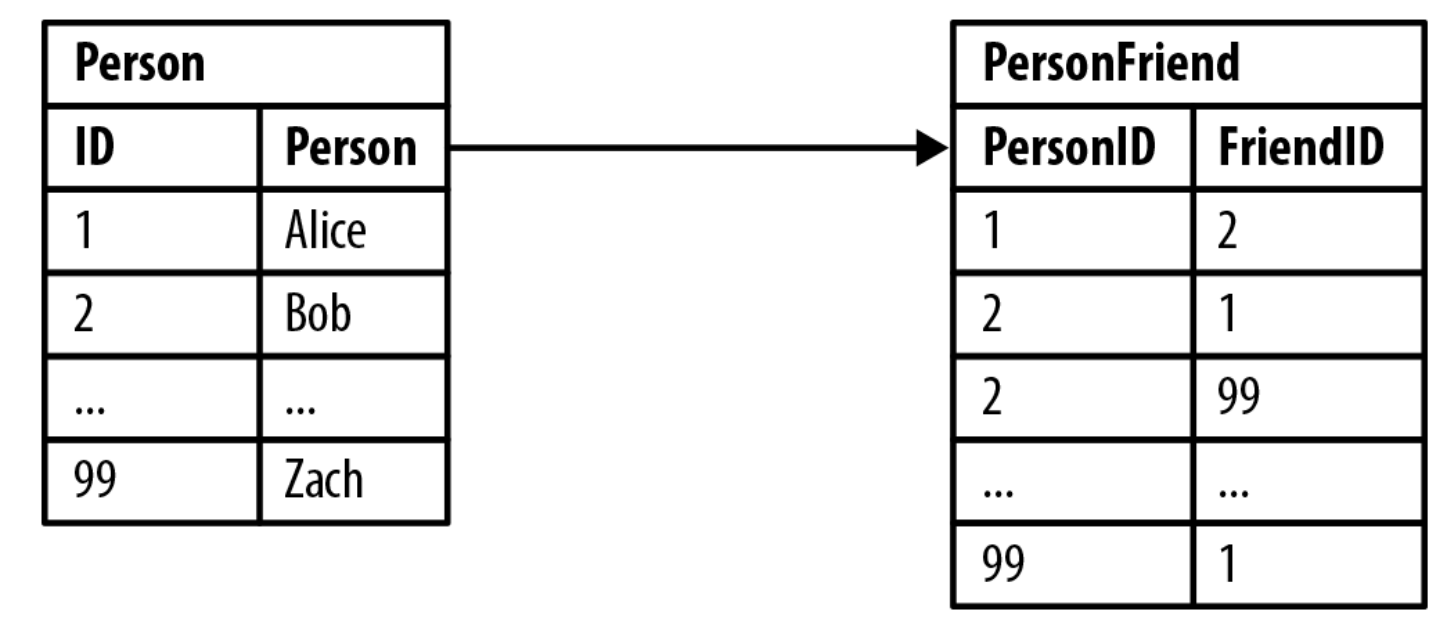
\includegraphics[width=.7\textwidth]{img/friends_table}
  \end{center}
\framebreak
\item Una consulta sencilla para obtener los amigos de Bob:
\begin{lstlisting}[language=SQL]
SELECT p1.Person
FROM Person p1 JOIN PersonFriend
ON PersonFriend.FriendID = p1.ID
JOIN Person p2
ON PersonFriend.PersonID = p2.ID
WHERE p2.Person = 'Bob'
\end{lstlisting}
\item Es sencilla y no es computacionalmente muy compleja
\item Como la relación de amistad no es recíproca siempre, a veces hay que
  hacer la búsqueda inversa:
\begin{lstlisting}[language=SQL]
SELECT p1.Person
FROM Person p1 JOIN PersonFriend
ON PersonFriend.PersonID = p1.ID
JOIN Person p2
ON PersonFriend.FriendID = p2.ID
WHERE p2.Person = 'Bob'
\end{lstlisting}
\item Esta consulta es más costosa que la anterior, porque se tienen que
  recorrer todas las filas de {\tt PersonFriend}

\item Pero ¿y si queremos ``{\bf los amigos de los amigos de Alice}''?
  Ahora la consulta es mucho más compleja computacionalmente y también más
  difícil de expresar en SQL:

\begin{lstlisting}[language=SQL]
SELECT p1.Person AS PERSON, p2.Person AS FRIEND_OF_FRIEND
FROM PersonFriend pf1 JOIN Person p1
ON pf1.PersonID = p1.ID
JOIN PersonFriend pf2
ON pf2.PersonID = pf1.FriendID
JOIN Person p2
ON pf2.FriendID = p2.ID
WHERE p1.Person = 'Alice' AND pf2.FriendID <> p1.ID
\end{lstlisting}

\item Y sólo estamos bajando un nivel (amigos de amigos de Alice)
\item Si tuviéramos que bajar otro nivel, se haría mucho más complejo por
  todos los {\tt JOIN}

\item En {\em Neo4j in Action\/}, Partner y Vukotic hicieron un experimento
  con Neo4j y MySQL con esta tabla
\item Buscaron amigos de amigos en diferentes niveles de profundidad
\item En una red de 1 millón de personas cada uno con unos~50~amigos

  \begin{small}
    \begin{tabular}{llll}
      \toprule
      Prof.& Tiempos RDBMS & Tiempos Neo4j & Resultados\\
      \midrule
      2&0,016&0,01&\~{}2500\\
      3&30,267&0,168&\~{}110.000\\
      4&1543,505&1,359&\~{}600.000\\
      5&(no termina)&2,132&\~{}800.000\\
      \bottomrule
    \end{tabular}
  \end{small}
\end{itemize}

\begin{center}
  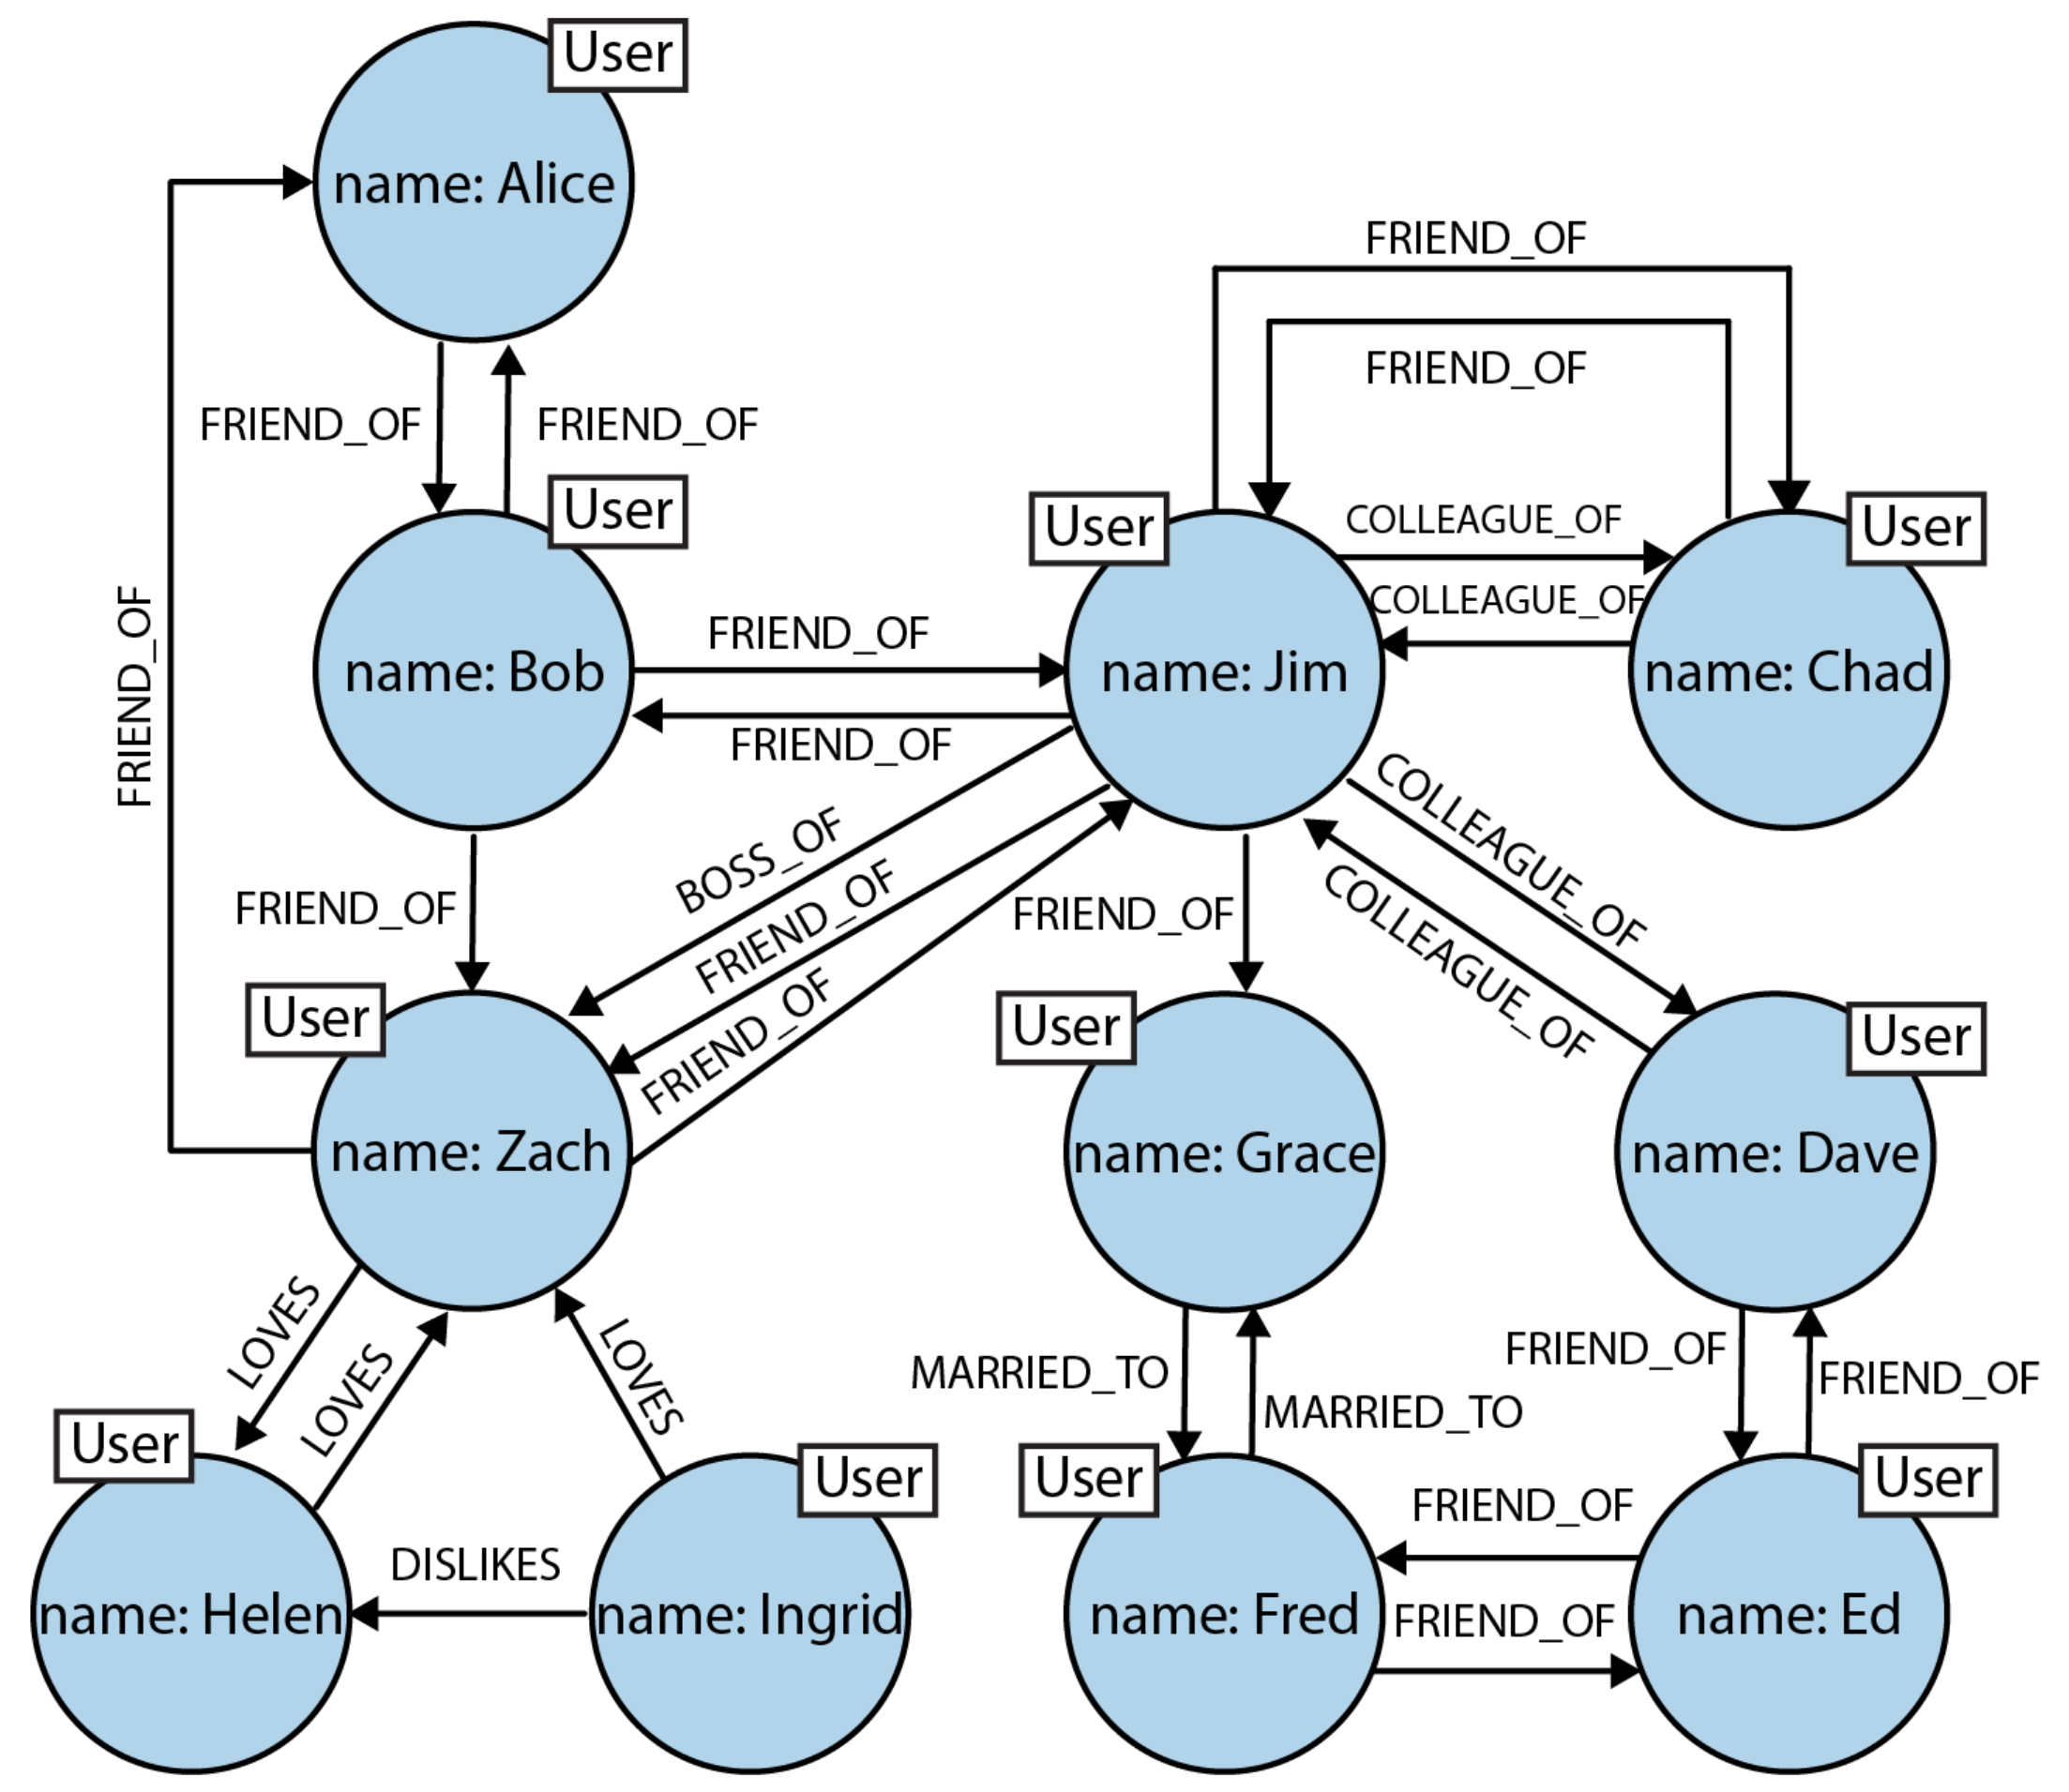
\includegraphics[width=.78\textwidth]{img/graph3}
\end{center}
\end{frame}

\subsubsection{Neo4j}

\begin{frame}
  \frametitle{Introducción a Neo4j}
\begin{itemize}
\item Ofrece una base de datos de grafos con posibilidad de extenderse a
  varios ordenadores (aunque sólo uno de los ordenadores soporta escritura,
  replicación {\em master}-{\em slave})
\item Es compatible con el estándar Apache TinkerPop para la creación de
  grafos
\item Ofrece un lenguaje de creación y consulta de grafos: {\bf Cypher}
\item Ofrece también un {\em browser\/} web para lanzar consultas
\item También una consola que interpreta el lenguaje Cypher
\item Se puede usar desde Jupyter Notebook con una extensión instalada en
  la máquina virtual
\item Finalmente, ofrece todos sus servicios a través de un API REST
  \end{itemize}
\end{frame}

\begin{frame}[allowframebreaks]
  \frametitle{Grafos en Neo4j}
  \begin{itemize}
  \item Los grafos en Neo4j son grafos etiquetados y con propiedades
  \item Están compuestos por {\bf nodos}, {\bf relaciones}, {\bf
      propiedades} y {\bf etiquetas}
\item Los nodos contienen propiedades, en la forma de pares clave-valor.
  Las claves son cadenas de caracteres y los valores pueden ser tipos
  primitivos o {\em arrays}
\item A los nodos se les puede etiquetar con una o más {\bfseries\itshape
    etiquetas}. Las etiquetas agrupan nodos por rol dentro del grafo
\item Las relaciones conectan nodos y estructuran el grafo. Una relación
  siempre tiene una dirección, un nombre propio, un nodo de inicio y otro
  de fin
\item Como los nodos, las relaciones también tienen propiedades. Esto
  permite añadir información adicional al hacer el recorrido, como el peso
  asociado a atravesar ese enlace o la calidad del mismo. Además ayudan a
  hacer más sencillas las consultas
  \end{itemize}
\end{frame}

% \subsection{Browser de Neo4j}

% \begin{frame}[fragile]
%   \frametitle{Inicio de Neo4j en la máquina virtual}
%   \begin{itemize}
%   \item Hay que establecer el número de ficheros abierto a 40.000 (si no
%     está ya en la máquina virtual):
% \item En el fichero {\tt /etc/security/limits.conf}, añadir:
% \begin{verbatim}
% vagrant    soft    nofile    40000
% vagrant    hard    nofile    40000
% \end{lstlisting}
% \item Y ejecutar, en el directorio {\em home\/} de {\tt vagrant}:
% \begin{verbatim}
% $ ./start-neo4j.sh
% \end{lstlisting}

% \item Y la consola:

% \begin{verbatim}
% $ neo4j/bin/neo4j-shell
% \end{lstlisting}
%   \end{itemize}
% \end{frame}

% \begin{frame}
%   \frametitle{Browser}
%   \url{http://127.0.0.1:7474}. Usuario: neo4j, pass: neo4j.\\
%  Cambiar {\em password\/} a ``neo''
% \includegraphics[width=\textwidth]{img/neo4jbrowser}
% \end{frame}

\subsubsection{El lenguaje Cypher}

\begin{frame}[fragile]
  \frametitle{El lenguaje Cypher}
  \begin{itemize}
\item Lenguaje de especificación de búsquedas y modificaciones en el
  grafo
\item En las búsquedas y creaciones de nodos se especifican nodos con la
  sintaxis:
\begin{lstlisting}[language=cypher]
( nombre:Etiqueta { propiedad: valor, ... } )
\end{lstlisting}

\item Las relaciones se especifican entre nodos de la siguiente manera,
  usando {\em ASCII art}:

\begin{lstlisting}[language=cypher]
(nodo_origen)-[:RELACIÓN]->(nodo_destino)
\end{lstlisting}
  \end{itemize}
\end{frame}

\begin{frame}[fragile]
  \frametitle{El lenguaje Cypher (ii)}
  \begin{itemize}
  \item Creación de nodos y enlaces: {\tt CREATE}
  \end{itemize}

\begin{lstlisting}[language=cypher]
CREATE (nodo1:Etiqueta1 { propX: valorX, ... } ),
       (nodo2:Etiqueta2 { propY: valorY, ... } ),
       ...
       (nodo1)-[:RELACIONADO_CON]->(nodo2)
\end{lstlisting}
\end{frame}

\begin{frame}[fragile,allowframebreaks]
  \frametitle{Consultas}
  \begin{itemize}
  \item Las consultas se realizan con el operador {\tt MATCH}
  \item Es un operador de consulta a través de ejemplos ({\em query by
      example})
\item Especifica nodos y propiedades como un ejemplo de los nodos y
  relaciones que se buscan
\item La sintaxis:

\begin{lstlisting}[language=cypher]
MATCH especificación, especificación, ...
[WHERE especificación]
RETURN [DISTINCT] nodos
\end{lstlisting}

\item {\tt MATCH} también se utiliza para seleccionar nodos para borrar
  ({\tt DELETE} o {\tt DETACH DELETE})

  \item Las consultas nombran nodos sobre los que se pueden buscar
    relaciones
\item Después, con {\tt RETURN} se especifica lo que devolver
\begin{lstlisting}[language=cypher]
MATCH (n:Post) RETURN n
\end{lstlisting}
(retorna todos los {\em posts})

\begin{lstlisting}[language=cypher]
MATCH (n { nombre: 'Diego' }) RETURN n.edad;
\end{lstlisting}

y también se puede especificar relaciones que se tienen que cumplir entre
los nodos para ser devueltos. Por ejemplo, todos los abuelos con sus
nietos:

\begin{lstlisting}[language=cypher]
MATCH (nieto), (abuelo),
   (nieto)-[:HIJO_DE]->()-[:HIJO_DE]->(abuelo)
 RETURN abuelo, nieto
\end{lstlisting}
o incluso:
\begin{lstlisting}[language=cypher]
MATCH (nieto)-[:HIJO_DE]->()-[:HIJO_DE]->(abuelo)
  RETURN abuelo, nieto
\end{lstlisting}

(nótense los nodos anónimos)
  \end{itemize}
\end{frame}

\begin{frame}[fragile]
  \frametitle{Creación de nodos a partir de otros}
  \begin{itemize}
  \item Un patrón común es la creación de nodos a partir de otros:
\item P. ej. apuntar los hijos de alguien:
\begin{lstlisting}[language=cypher]
MATCH (padre:Persona { nombre: 'Diego' })
 CREATE (violeta:Persona {nombre: 'Violeta'}),
        (martina:Persona {nombre: 'Martina'}),
        (violeta)-[:HIJO_DE]->(padre),
        (martina)-[:HIJO_DE]->(padre)
\end{lstlisting}
  \end{itemize}
\end{frame}

\begin{frame}[fragile]
  \frametitle{Creación de relaciones}
  \begin{itemize}
  \item Para crear sólo relaciones y mezclar los nodos que ya existan se
    suele utilizar {\tt MERGE}
\item P. ej. si alguna de mis hijas existe, no se crea. Sólo se crean las
  que no existen
\begin{lstlisting}[language=cypher]
MATCH (padre:Persona { nombre: 'Diego' })
 MERGE (violeta:Persona {nombre: 'Violeta'}),
        (martina:Persona {nombre: 'Martina'}),
        (violeta)-[:HIJO_DE]->(padre),
        (martina)-[:HIJO_DE]->(padre)
\end{lstlisting}
  \end{itemize}
\end{frame}


\begin{frame}[fragile]
  \frametitle{Índices}
  \begin{itemize}
  \item Se pueden crear índices para búsquedas rápidas sobre atributos:
\begin{lstlisting}[language=cypher]
CREATE INDEX ON :Etiqueta(nombre)
\end{lstlisting}
  \end{itemize}
\end{frame}



\subsection{Arrays}

\begin{frame}
  \frametitle{Bases de Datos basadas en Arrays}
  \begin{itemize}
\item Suelen presentarse como bases de datos que soportan SQL y añaden
  operaciones para trabajar con conjuntos de datos especiales (arrays)
\item Utilizadas para tratamiento de grandes cantidades de datos de forma
  estadística o de modelado y OLAP
\item Soportan también datos geográficos, ya que pueden definir rangos
  numéricos de una o varias dimensiones (2D para cálculos geográficos)
\item Ejemplos: MonetDB, SciDB, rasdaman
  \end{itemize}
\end{frame}

\section{Referencias}

\begin{frame}[fragile,allowframebreaks]
  \frametitle{Referencias}

\begin{thebibliography}{Paternostro, 2009}

\setbeamertemplate{bibliography item}[book]
\bibitem[Marz, 2015]{Marz2015}
Nathan Marz, James Warren
\newblock {\em Big Data: Principles and best
  practices of scalable realtime data systems}
\newblock Manning Publications,~2015

\bibitem[Redmond, 2012]{Redmond2012}
Eric Redmond, Jim R. Wilson
\newblock {\em Seven Databases in Seven Weeks: A Guide to Modern Databases
  and the NoSQL Movement}
\newblock Pragmatic  Bookshelf,~2012

\bibitem[Sadalage, 2013]{Sadalage2013}
Pramod J. Saldage, Martin Fowler
\newblock {\em NoSQL Distilled. A Brief Guide to the Emerging World of
  Polyglot Persistence}
\newblock Addison-Wesley,~2013

\bibitem[Wilson, 2012]{Wilson2012}
Jim R. Wilson, Eric Redmond
\newblock {\em Seven Databases in Seven Weeks}

\bibitem[Kleppmann, 2016]{Kleppmann2016}
Kleppmann
\newblock  \emph{Designing Data Intensive Applications}

\bibitem[George, 2011]{George2011}
Lars George
\newblock {\em HBase, The Definitive Guide}

\setbeamertemplate{bibliography item}[online]
\bibitem[ApacheHBaseTeam, 2016]{ApacheHBaseTeam2016}
  The Apache HBase Team
  \newblock {\em Apache HBase Reference Guide}
  \newblock \url{https://hbase.apache.org/book.html}

\bibitem[HBaseCon, 2012a]{HBaseCon2012a}
  Ian Varley
\newblock Vídeo: {\em HBase Schema Design}
\newblock
\url{http://www.cloudera.com/content/dam/www/marketing/resources/events/hbase-con/video-hbasecon-2012-hbasecon-2012.png.landing.html}
\newblock Transparencias:
\url{http://es.slideshare.net/ivarley/hbase-schema-design-hbasecon-2012}

\bibitem[George, 2013]{George2013}
  Lars George
\newblock {\em HBase Schema Design}
\newblock \url{https://2013.nosql-matters.org/cgn/wp-content/uploads/2013/05/HBase-Schema-Design-NoSQL-Matters-April-2013.pdf}
\newblock Otro vídeo: \url{https://vimeo.com/44715954}
\newblock Sus transparencias: \url{http://2012.berlinbuzzwords.de/sites/2012.berlinbuzzwords.de/files/slides/hbase-lgeorge-bbuzz12.pdf}

\bibitem[Khurana, 2013]{khurana2013}
Amandeep Khurana, ;login:
\newblock {\em Introduction to HBase Schema Design}
\newblock \url{http://0b4af6cdc2f0c5998459-c0245c5c937c5dedcca3f1764ecc9b2f.r43.cf2.rackcdn.com/9353-login1210_khurana.pdf}

\bibitem[McDonald, 2015]{mcdonald2015}
  Carol McDonald
  \newblock {\em Guidelines for HBase Schema Design}
  \newblock \url{https://www.mapr.com/blog/guidelines-hbase-schema-design}

\end{thebibliography}
\end{frame}


\end{document}

%%% Local variables:
%%% mode: LaTeX
%%% TeX-master: t
%%% ispell-local-dictionary: "spanish"
%%% fill-column: 75
%%% TeX-parse-self: t
%%% TeX-auto-save: t
%%% End:
%%% vim: expandtab shiftwidth=2 tabstop=2
